\documentclass[11pt]{article}\usepackage[]{graphicx}\usepackage[]{color}
%% maxwidth is the original width if it is less than linewidth
%% otherwise use linewidth (to make sure the graphics do not exceed the margin)
\makeatletter
\def\maxwidth{ %
  \ifdim\Gin@nat@width>\linewidth
    \linewidth
  \else
    \Gin@nat@width
  \fi
}
\makeatother

\definecolor{fgcolor}{rgb}{0.345, 0.345, 0.345}
\newcommand{\hlnum}[1]{\textcolor[rgb]{0.686,0.059,0.569}{#1}}%
\newcommand{\hlstr}[1]{\textcolor[rgb]{0.192,0.494,0.8}{#1}}%
\newcommand{\hlcom}[1]{\textcolor[rgb]{0.678,0.584,0.686}{\textit{#1}}}%
\newcommand{\hlopt}[1]{\textcolor[rgb]{0,0,0}{#1}}%
\newcommand{\hlstd}[1]{\textcolor[rgb]{0.345,0.345,0.345}{#1}}%
\newcommand{\hlkwa}[1]{\textcolor[rgb]{0.161,0.373,0.58}{\textbf{#1}}}%
\newcommand{\hlkwb}[1]{\textcolor[rgb]{0.69,0.353,0.396}{#1}}%
\newcommand{\hlkwc}[1]{\textcolor[rgb]{0.333,0.667,0.333}{#1}}%
\newcommand{\hlkwd}[1]{\textcolor[rgb]{0.737,0.353,0.396}{\textbf{#1}}}%
\let\hlipl\hlkwb

\usepackage{framed}
\makeatletter
\newenvironment{kframe}{%
 \def\at@end@of@kframe{}%
 \ifinner\ifhmode%
  \def\at@end@of@kframe{\end{minipage}}%
  \begin{minipage}{\columnwidth}%
 \fi\fi%
 \def\FrameCommand##1{\hskip\@totalleftmargin \hskip-\fboxsep
 \colorbox{shadecolor}{##1}\hskip-\fboxsep
     % There is no \\@totalrightmargin, so:
     \hskip-\linewidth \hskip-\@totalleftmargin \hskip\columnwidth}%
 \MakeFramed {\advance\hsize-\width
   \@totalleftmargin\z@ \linewidth\hsize
   \@setminipage}}%
 {\par\unskip\endMakeFramed%
 \at@end@of@kframe}
\makeatother

\definecolor{shadecolor}{rgb}{.97, .97, .97}
\definecolor{messagecolor}{rgb}{0, 0, 0}
\definecolor{warningcolor}{rgb}{1, 0, 1}
\definecolor{errorcolor}{rgb}{1, 0, 0}
\newenvironment{knitrout}{}{} % an empty environment to be redefined in TeX

\usepackage{alltt}
\usepackage[utf8]{inputenc}
\usepackage{amsmath}
\usepackage{amsfonts}
\usepackage{amscd}
\usepackage{amssymb}
\usepackage{natbib}
%\usepackage{fullpage}
\usepackage{url}
\usepackage{graphicx,times}
\usepackage{setspace}
\usepackage{ragged2e}

\usepackage{geometry}
\geometry{margin=1in}
\IfFileExists{upquote.sty}{\usepackage{upquote}}{}
\begin{document}

\begin{center}

\noindent {\huge \bf Supporting data analysis for 
  ``Challenging nostalgia and performance metrics in baseball''} \\

\vspace{.2in}

Daniel J. Eck

\vspace{.01in}

\textit{Department of Statistics, University of Illinois Urbana-Champaign \\ 
email: \url{dje13@illinois.edu}}

\vspace{.1in}

\end{center}

\begin{abstract}
We show that the great baseball players that started their 
careers before 1950 are overrepresented among rankings of baseball's all time 
greatest players.  The year 1950 coincides with the decennial US Census that 
is closest to when Major League Baseball (MLB) was integrated in 1947. 
We also show that performance metrics used to compare players have substantial 
era biases that favor players who started their careers before 1950. 
In showing that the these players are overrepresented, no individual 
statistics or era adjusted metrics are used.  Instead, we argue that the eras 
in which players played are fundamentally different and are not comparable.  
In particular, there were significantly fewer MLB eligible players available 
at and before 1950.  As a consequence of this and other differences across 
eras, we argue that popular opinion, performance metrics, and expert opinion 
over include players that started their careers before 1950 in their rankings 
of baseball's all time greatest players. 
\end{abstract}

%\noindent{\bf Keywords}: Sabermetrics, binomial distribution, 
%population dynamics, baseball ranking, era confounding \\

\section*{Creating this document}

The purpose of this document is to make transparent the analysis in 
\citet{eck2019challenging}.  All calculations and tables that appear in 
\citet{eck2019challenging} are displayed in this document.  
This document is a technical report that can be compiled by anyone with a 
computer who has the UN Census data file,
\begin{center}
\begin{verbatim}
  WPP2010_DB4_F2A_POPULATION_BY_AGE_MALE_ANNUAL_1950-2010.csv
\end{verbatim}
\end{center}
This file is located at \url{https://population.un.org/wpp/Download/Standard/Population/}. 
The relevant file is the population by age groups - male .xls file under the 
age composition sub group.  The corresponding .csv file is included on the 
author's GitHub page along with this technical report.  





\section{Introduction}
%\doublespacing
It is easy to be blown away by the accomplishments of great old time 
baseball players when you look at their raw or advanced baseball statistics.  
%% Consider making a chart for the mind-boggling seasons and careers.
These players produced mind-boggling numbers. For example, see 
Babe Ruth's batting average and pitching numbers, 
%Honus Wagner's 1900 season, 
Ty Cobb's 1911 season, 
Walter Johnson's 1913 season, 
Tris Speaker's 1916 season, 
Rogers Hornsby's 1925 season, 
and
Lou Gehrig's 1931 season.
The statistical feats achieved by these players (and others) far surpass 
the statistics that recent and current players produce.  At first glance 
it seems that players from the old eras were vastly superior to the 
players in more modern eras, but is this true? 
%Were the old timers actually better? 
In this paper, we investigate whether baseball players from earlier 
eras of professional baseball are overrepresented among the game's all-time 
greatest players according to popular opinion, performance metrics, and expert 
opinion.  We define baseball players from earlier eras to be those that 
started their MLB careers in the 1950 season or before.  
This year is chosen because it coincides with the decennial US Census 
and is close to 1947, the year in which baseball became integrated. 

In this paper we do not compare baseball players via their statistical 
accomplishments.  Such measures exhibit era biases that are confounded with 
actual performance.  Consider the single season homerun record as an example. 
Before Babe Ruth, the single season homerun record was 27 by Ned Williamson in 
1884. %\citep{reichler1985encyclopedia}.  
Babe Ruth broke this record in 1919 
when he hit 29 homeruns.  He subsequently destroyed his own record in 
the following 1920 season when he hit 54 homeruns.  The runner up in 1920 
finished the season with a grand total of 15 homeruns.  At this point in time 
homerun hitting was not an integral part of a batter's approach. %\citep{bref}.  
This has changed. Now, we often see multiple batters reach at least 30-40 
homeruns within one season and a 50 homerun season is not a rare 
occurrence. %\citep{bref, fangraphs}. 
In the 1920s, Babe Ruth stood head and shoulders above his peers due to a 
combination of his innate talent and circumstance.  
His approach was quickly emulated and became widely adopted. %\citep{bref}.  
However, Ruth's accomplishments as a homerun hitter would not stand out nearly 
as much if he played today and put up similar homerun totals.    
The example of homeruns hit by Babe Ruth and the impact they had relative 
to his peers represents a case where adjustment towards a peer-derived 
baseline fails across eras.  No one reasonably expects 1920 Babe Ruth to hit 
more than three times the amount of homeruns hit by the second best homerun 
hitter if the 1920 version of Babe Ruth played today.  
This is far from an isolated case.  

There are several statistical approaches currently used to compare baseball 
players across eras. 
These include 
wins above replacement as calculated by baseball reference (bWAR), %\citep{bref}, 
wins above replacement as calculated by fangraphs (fWAR), %\citep{fangraphs}, 
adjusted OPS+, %\citep{bref, fangraphs},
adjusted ERA+, %\citep{bref, fangraphs},
era-adjusted detrending \citep{petersen}, 
computing normal scores as in Jim Albert's work on a Baseball Statistics Course 
in the Journal of Statistics Education, 
and era bridging \citep{berry1999eras}. 
A number of these are touted to be season adjusted and the remainder are 
widely understood to have the same effect.  
In one way or another all of these statistical approaches compare the  
accomplishments of players within one season to a baseline that 
is computed from statistical data within that same season.  
This method of player comparison ignores talent discrepancies that exist across 
seasons as noted by Stephen J. Gould in numerous lectures and papers.
%\citet{gould1996fullhouse, schmidt2005concentration}.  
Currently, there is no definitive quantitative or qualitative basis for 
comparing these baselines, which are used to form intra-season player 
comparisons, across seasons.  These methods therefore fail to properly 
compare players across eras of baseball despite the claim that they are 
season adjusted.  

Worse still is that these approaches exhibit a favorable bias towards baseball 
players who played in earlier seasons 
\citep{schmidt2005concentration}.  
We explore this bias from two separate theoretical perspectives underlying how 
baseball players from different eras would actually compete against each 
other.  The first perspective is that players would teleport across eras to 
compete against each other.  From this perspective, the players from earlier eras 
are at a competitive disadvantage because, on average, baseball players have 
gotten better as time has progressed.
%\citep{gould1996fullhouse, schmidt2005concentration}.  
Specifically, it is widely acknowledged that 
fastball velocity, pitch repertoire, training methods, and management 
strategies have all improved over time   
%\citep{lewis2004moneyball, keh2013offseason, thorn2014pitching, 
%doran2015velocity, arthur2016bullpen, castrovince2016velocity}.  
We do not find the teleportation perspective to be of 
much interest for these reasons.  The second perspective is that a player from 
one era could adapt naturally to the game conditions of another era if they 
grew up in that time. 
This line of thinking is challenging to current statistical methodology because 
adjustment to a peer-derived baseline no longer makes sense. 
Even in light of these challenges with the second perspective, we find that the 
players from earlier eras are overrepresented among baseball's all time greats.  
We justify our findings through the consideration of population dynamics which 
have changed drastically over time.  %\citep{gould1996fullhouse}. \\



\section{Data}

The MLB eligible population is not well-defined.  As a proxy, we can say 
that the MLB eligible population is the decennial count of males aged 
20-29 that are living in the United States (US) and Canada. 
Baseball was segregated on racial grounds until 1947.  As a result, 
African American and Hispanic American population counts in the US  
and Canada are added to our dataset starting in 1960.  The year 1960 is chosen 
because the integration of the MLB was slow as noted in Armour's work on the 
integration of baseball in the Society for American Baseball Research.

Players from Central and South American countries and the Caribbean islands 
were also targets of discrimination.
We have added data from these countries to the MLB eligible population starting 
in 1960:
%The countries included in our dataset are 
Mexico, 
the Dominican Republic, 
Venezuela, 
Cuba, 
Panama, 
Puerto Rico, 
Netherlands Antilles, 
Aruba, 
Honduras, 
Jamaica, 
the Bahamas, 
Peru, 
Columbia, 
Nicaragua, 
and the United States Virgin Islands.  
In the mid to late 1990s, the MLB and minors saw an influx of Asian baseball 
players from Japan, South Korea, Taiwan, and the Philippines.  
We have added the populations of these countries to the MLB eligible population 
starting in 2000.  In 2010, the MLB established a national training center in 
Brazil as noted in Lor{\'e}'s work on the popularity of baseball in Brazil in 
the Culture Trip.  Therefore, we have included the Brazilian population of 
20-24 year old men into our MLB eligible population starting in 2010.  
We estimate that the 2011-2015 MLB eligible population is half of the 
MLB eligible population counted in the 2010 decennial Censuses.  We expect 
that this underestimates the actual 2011-2015 MLB eligible population 
since we have observed a constant increase in the overall MLB eligible 
population as time increases. 

We now load in the UN population dataset and begin constructing the population 
dataset used in our analysis.

\begin{knitrout}
\definecolor{shadecolor}{rgb}{0.969, 0.969, 0.969}\color{fgcolor}\begin{kframe}
\begin{alltt}
\hlcom{# load in UN dataset and remove irrelevant variables}
\hlkwd{options}\hlstd{(}\hlkwc{warn}\hlstd{=}\hlopt{-}\hlnum{1}\hlstd{)}
\hlstd{WPP2010} \hlkwb{<-}
  \hlkwd{read.csv}\hlstd{(}\hlstr{"WPP2010_DB4_F2A_POPULATION_BY_AGE_MALE_ANNUAL_1950-2010.csv"}\hlstd{,}
  \hlkwc{header} \hlstd{=} \hlnum{TRUE}\hlstd{)}
\hlkwd{colnames}\hlstd{(WPP2010)[}\hlnum{3}\hlstd{]} \hlkwb{<-} \hlkwd{c}\hlstd{(}\hlstr{"region"}\hlstd{)}
\hlkwd{colnames}\hlstd{(WPP2010)[}\hlnum{6}\hlstd{]} \hlkwb{<-} \hlkwd{c}\hlstd{(}\hlstr{"year"}\hlstd{)}
\hlkwd{colnames}\hlstd{(WPP2010)[}\hlnum{7}\hlopt{:}\hlnum{17}\hlstd{]} \hlkwb{<-} \hlkwd{paste}\hlstd{(}\hlstr{"age"}\hlstd{,} \hlnum{0}\hlopt{:}\hlnum{10} \hlopt{*} \hlnum{5}\hlstd{,} \hlkwc{sep} \hlstd{=} \hlstr{""}\hlstd{)}
\hlstd{WPP2010} \hlkwb{<-} \hlstd{WPP2010[,} \hlkwd{c}\hlstd{(}\hlnum{3}\hlstd{,} \hlnum{6}\hlstd{,} \hlnum{11}\hlstd{,} \hlnum{12}\hlstd{)]}

\hlcom{# restrict attention to countries of interest}
\hlstd{countries} \hlkwb{<-} \hlkwd{c}\hlstd{(}\hlstr{"Mexico"}\hlstd{,} \hlstr{"Aruba"}\hlstd{,} \hlstr{"Panama"}\hlstd{,}
  \hlstr{"Columbia"}\hlstd{,} \hlstr{"Cuba"}\hlstd{,} \hlstr{"Honduras"}\hlstd{,} \hlstr{"Jamaica"}\hlstd{,}
  \hlstr{"Bahamas"}\hlstd{,} \hlstr{"Peru"}\hlstd{,} \hlstr{"Dominican Republic"}\hlstd{,}
  \hlstr{"Netherlands Antilles"}\hlstd{,} \hlstr{"Puerto Rico"}\hlstd{,}
  \hlstr{"Venezuela (Bolivarian Republic of)"}\hlstd{,} \hlstr{"Nicaragua"}\hlstd{,}
  \hlstr{"United States Virgin Islands"}\hlstd{,} \hlstr{"Canada"}\hlstd{,}
  \hlstr{"United States of America"}\hlstd{)}

\hlcom{# obtain population data for all countries for all years}
\hlstd{dataset} \hlkwb{<-} \hlstd{WPP2010[WPP2010[,} \hlnum{1}\hlstd{]} \hlopt \hlstd{countries, ]}
\hlstd{dataset[,} \hlnum{3}\hlstd{]} \hlkwb{<-} \hlkwd{as.numeric}\hlstd{(}\hlkwd{levels}\hlstd{(dataset[,} \hlnum{3}\hlstd{]))[dataset[,} \hlnum{3}\hlstd{]]}
\hlstd{dataset[,} \hlnum{4}\hlstd{]} \hlkwb{<-} \hlkwd{as.numeric}\hlstd{(}\hlkwd{levels}\hlstd{(dataset[,} \hlnum{4}\hlstd{]))[dataset[,} \hlnum{4}\hlstd{]]}
\hlstd{dataset[,} \hlnum{3}\hlopt{:}\hlnum{4}\hlstd{]} \hlkwb{<-} \hlstd{dataset[,} \hlnum{3}\hlopt{:}\hlnum{4}\hlstd{]} \hlopt{/} \hlnum{1000}

\hlcom{# get population dataset for this analysis corresponding to the }
\hlcom{# Census years }
\hlstd{dataset.years} \hlkwb{<-} \hlstd{dataset[dataset[,} \hlnum{2}\hlstd{]} \hlopt
  \hlkwd{c}\hlstd{(}\hlstr{"1960"}\hlstd{,} \hlstr{"1970"}\hlstd{,} \hlstr{"1980"}\hlstd{,} \hlstr{"1990"}\hlstd{,} \hlstr{"2000"}\hlstd{,} \hlstr{"2010"}\hlstd{), ]}
\hlstd{dataset.years[,} \hlnum{2}\hlstd{]} \hlkwb{<-} \hlkwd{factor}\hlstd{(dataset.years[,} \hlnum{2}\hlstd{])}
\hlstd{dataset.years.list} \hlkwb{<-} \hlkwd{split}\hlstd{(dataset.years,} \hlkwc{f} \hlstd{=} \hlkwd{as.factor}\hlstd{(dataset.years[,} \hlnum{2}\hlstd{]))}
\hlstd{pops} \hlkwb{<-} \hlkwd{unlist}\hlstd{(}\hlkwd{lapply}\hlstd{(dataset.years.list,} \hlkwa{function}\hlstd{(}\hlkwc{x}\hlstd{)} \hlkwd{sum}\hlstd{(x[,} \hlnum{3}\hlopt{:}\hlnum{4}\hlstd{])))}
\end{alltt}
\end{kframe}
\end{knitrout}

We now add in the Taiwan population figures from the CIA World Factbook.  
The CIA World Factbook does not provide population data for men aged 
20-29 for 2000 or 2010.  It does provide estimated population data for 
men aged 15-24 for 2018.  We will use this estimate as the estimate of 
the Taiwan male population aged 20-29 for 2000 or 2010.

\begin{knitrout}
\definecolor{shadecolor}{rgb}{0.969, 0.969, 0.969}\color{fgcolor}\begin{kframe}
\begin{alltt}
\hlcom{#approximation from CIA World Factbook at }
\hlcom{#https://www.cia.gov/library/publications/the-world-factbook/geos/print_tw.html}
\hlstd{dataTaiwan2000} \hlkwb{<-} \hlnum{1.50}
\hlstd{dataTaiwan2010} \hlkwb{<-} \hlnum{1.50}
\hlstd{pops[}\hlnum{5}\hlstd{]} \hlkwb{<-} \hlstd{pops[}\hlnum{5}\hlstd{]} \hlopt{+} \hlstd{dataTaiwan2000}
\hlstd{pops[}\hlnum{6}\hlstd{]} \hlkwb{<-} \hlstd{pops[}\hlnum{6}\hlstd{]} \hlopt{+} \hlstd{dataTaiwan2010}
\end{alltt}
\end{kframe}
\end{knitrout}

We now add in the US and Canadian population data for the Census years from 
1880-1950.  Note that the Canadian Census is recorded one year after the 
US Census.  A precise Canadian Census exists for males aged 20-30 for the 
years 1881, 1891, and 1901.  We use this information to estimate the 
proportion of Canadian males aged 20-30 from 1911-1951 for which 
an accurate count of Canadian males aged 20-30 was not easy to find.  

\begin{knitrout}
\definecolor{shadecolor}{rgb}{0.969, 0.969, 0.969}\color{fgcolor}\begin{kframe}
\begin{alltt}
\hlcom{## Canadian population before 1960}
\hlcom{#https://www65.statcan.gc.ca/acyb02/1907/acyb02_1907001701a-eng.htm}
\hlstd{Can1881} \hlkwb{<-} \hlnum{0.21} \hlopt{+} \hlnum{0.17}
\hlcom{#https://www65.statcan.gc.ca/acyb02/1907/acyb02_1907001701a-eng.htm}
\hlstd{Can1891} \hlkwb{<-} \hlnum{0.24} \hlopt{+} \hlnum{0.19}
\hlcom{#https://www65.statcan.gc.ca/acyb02/1907/acyb02_1907001701a-eng.htm}
\hlstd{Can1901} \hlkwb{<-} \hlnum{0.26} \hlopt{+} \hlnum{0.22}
\hlcom{#https://www65.statcan.gc.ca/acyb02/1947/acyb02_19470113009-eng.htm}
\hlstd{CanM1881} \hlkwb{<-} \hlnum{2.19}
\hlcom{#https://www65.statcan.gc.ca/acyb02/1947/acyb02_19470113009-eng.htm}
\hlstd{CanM1891} \hlkwb{<-} \hlnum{2.16}
\hlcom{#https://www65.statcan.gc.ca/acyb02/1947/acyb02_19470113009-eng.htm}
\hlstd{CanM1901} \hlkwb{<-} \hlnum{2.75}
\hlstd{propCan2030} \hlkwb{<-} \hlstd{(Can1881} \hlopt{+} \hlstd{Can1891} \hlopt{+} \hlstd{Can1901)} \hlopt{/}
  \hlstd{(CanM1881} \hlopt{+} \hlstd{CanM1891} \hlopt{+} \hlstd{CanM1901)}
\hlcom{#https://www65.statcan.gc.ca/acyb02/1947/acyb02_19470113009-eng.htm}
\hlstd{Can1911} \hlkwb{<-} \hlnum{3.82} \hlopt{*} \hlstd{propCan2030}
\hlcom{#https://www65.statcan.gc.ca/acyb02/1947/acyb02_19470113009-eng.htm}
\hlstd{Can1921} \hlkwb{<-} \hlnum{4.53} \hlopt{*} \hlstd{propCan2030}
\hlcom{#https://www65.statcan.gc.ca/acyb02/1947/acyb02_19470113009-eng.htm}
\hlstd{Can1931} \hlkwb{<-} \hlnum{5.37} \hlopt{*} \hlstd{propCan2030}
\hlcom{#https://www65.statcan.gc.ca/acyb02/1947/acyb02_19470113009-eng.htm}
\hlstd{Can1941} \hlkwb{<-} \hlnum{5.90} \hlopt{*} \hlstd{propCan2030}
\hlcom{#https://www65.statcan.gc.ca/acyb02/1967/acyb02_19670194010-eng.htm}
\hlstd{Can1951} \hlkwb{<-} \hlnum{7.09} \hlopt{*} \hlstd{propCan2030}

\hlcom{## US population before 1960}
\hlcom{#https://www2.census.gov/library/publications/decennial/1880/vol-01-population/1880_v1-15.pdf}
\hlstd{US1880} \hlkwb{<-} \hlnum{2.22} \hlopt{+} \hlnum{1.84}
\hlcom{#https://www2.census.gov/library/publications/decennial/1900/volume-2/volume-2-p5.pdf}
\hlstd{US1900} \hlkwb{<-} \hlnum{2.73} \hlopt{+} \hlnum{2.37}
\hlstd{US1890} \hlkwb{<-} \hlkwd{mean}\hlstd{(}\hlkwd{c}\hlstd{(US1880,US1900))}
\hlcom{#https://www2.census.gov/library/publications/decennial/1910/volume-1/volume-1-p6.pdf}
\hlstd{US1910} \hlkwb{<-} \hlnum{4.07} \hlopt{+} \hlnum{3.79}
\hlcom{#https://www2.census.gov/library/publications/decennial/1920/volume-2/41084484v2ch03.pdf}
\hlstd{US1920} \hlkwb{<-} \hlnum{4.02} \hlopt{+} \hlnum{4.09}
\hlcom{#https://www2.census.gov/library/publications/decennial/1930/population-volume-2/16440598v2ch11.pdf}
\hlstd{US1930} \hlkwb{<-} \hlnum{4.69} \hlopt{+} \hlnum{4.25}
\hlcom{#https://www2.census.gov/library/publications/decennial/1940/population-volume-4/33973538v4p1ch1.pdf}
\hlstd{US1940} \hlkwb{<-} \hlnum{1.08} \hlopt{+} \hlnum{1.06} \hlopt{+} \hlnum{1.01} \hlopt{+} \hlnum{1.00} \hlopt{+} \hlnum{1.01} \hlopt{+}
  \hlnum{1.01} \hlopt{+} \hlnum{0.99} \hlopt{+} \hlnum{0.98} \hlopt{+} \hlnum{0.97} \hlopt{+} \hlnum{0.95}
\hlcom{#https://www2.census.gov/library/publications/decennial/1950/population-volume-2/21983999v2p1ch2.pdf}
\hlstd{US1950} \hlkwb{<-} \hlnum{5.00} \hlopt{+} \hlnum{5.30}
\end{alltt}
\end{kframe}
\end{knitrout}

We now add the Japan, South Korea, and Philippines population for men aged 
20-29 for 2000 or 2010 and the 2010 Brazil population for men aged 20-24 to 
the population dataset.   

\begin{knitrout}
\definecolor{shadecolor}{rgb}{0.969, 0.969, 0.969}\color{fgcolor}\begin{kframe}
\begin{alltt}
\hlcom{# load in UN dataset and remove irrelevant variables}
\hlkwd{options}\hlstd{(}\hlkwc{warn}\hlstd{=}\hlopt{-}\hlnum{1}\hlstd{)}
\hlstd{WPP2010} \hlkwb{<-}
  \hlkwd{read.csv}\hlstd{(}\hlstr{"WPP2010_DB4_F2A_POPULATION_BY_AGE_MALE_ANNUAL_1950-2010.csv"}\hlstd{,}
  \hlkwc{header} \hlstd{=} \hlnum{TRUE}\hlstd{)}
\hlkwd{colnames}\hlstd{(WPP2010)[}\hlnum{3}\hlstd{]} \hlkwb{<-} \hlkwd{c}\hlstd{(}\hlstr{"region"}\hlstd{)}
\hlkwd{colnames}\hlstd{(WPP2010)[}\hlnum{6}\hlstd{]} \hlkwb{<-} \hlkwd{c}\hlstd{(}\hlstr{"year"}\hlstd{)}
\hlkwd{colnames}\hlstd{(WPP2010)[}\hlnum{7}\hlopt{:}\hlnum{17}\hlstd{]} \hlkwb{<-} \hlkwd{paste}\hlstd{(}\hlstr{"age"}\hlstd{,} \hlnum{0}\hlopt{:}\hlnum{10} \hlopt{*} \hlnum{5}\hlstd{,} \hlkwc{sep} \hlstd{=} \hlstr{""}\hlstd{)}
\hlstd{WPP2010} \hlkwb{<-} \hlstd{WPP2010[,} \hlkwd{c}\hlstd{(}\hlnum{3}\hlstd{,} \hlnum{6}\hlstd{,} \hlnum{11}\hlstd{,} \hlnum{12}\hlstd{)]}

\hlcom{# get population data for relevant countries }
\hlstd{countries} \hlkwb{<-} \hlkwd{c}\hlstd{(}\hlstr{"Brazil"}\hlstd{,} \hlstr{"Japan"}\hlstd{,} \hlstr{"Philippines"}\hlstd{,} \hlstr{"Republic of Korea"}\hlstd{)}
\hlstd{dataset} \hlkwb{<-} \hlstd{WPP2010[WPP2010[,} \hlnum{1}\hlstd{]} \hlopt \hlstd{countries, ]}
\hlstd{dataset[,} \hlnum{3}\hlstd{]} \hlkwb{<-} \hlkwd{as.numeric}\hlstd{(}\hlkwd{levels}\hlstd{(dataset[,} \hlnum{3}\hlstd{]))[dataset[,} \hlnum{3}\hlstd{]]}
\hlstd{dataset[,} \hlnum{4}\hlstd{]} \hlkwb{<-} \hlkwd{as.numeric}\hlstd{(}\hlkwd{levels}\hlstd{(dataset[,} \hlnum{4}\hlstd{]))[dataset[,} \hlnum{4}\hlstd{]]}
\hlstd{dataset[,} \hlnum{3}\hlopt{:}\hlnum{4}\hlstd{]} \hlkwb{<-} \hlstd{dataset[,} \hlnum{3}\hlopt{:}\hlnum{4}\hlstd{]} \hlopt{/} \hlnum{1000}

\hlcom{# get population dataset for this analysis corresponding to the }
\hlcom{# Census years }
\hlstd{dataset.years} \hlkwb{<-} \hlstd{dataset[dataset[,} \hlnum{2}\hlstd{]} \hlopt \hlkwd{c}\hlstd{(}\hlstr{"2000"}\hlstd{,} \hlstr{"2010"}\hlstd{), ]}
\hlstd{dataset.years[,} \hlnum{2}\hlstd{]} \hlkwb{<-} \hlkwd{factor}\hlstd{(dataset.years[,} \hlnum{2}\hlstd{])}
\hlcom{# Brazil age 20-24, year 2010}
\hlstd{Brazil2010} \hlkwb{<-} \hlkwd{round}\hlstd{(dataset.years[}\hlnum{8}\hlstd{,} \hlnum{3}\hlstd{],} \hlnum{2}\hlstd{)}
\hlstd{dataset.years} \hlkwb{<-} \hlstd{dataset.years[}\hlkwd{c}\hlstd{(}\hlnum{1}\hlopt{:}\hlnum{3}\hlstd{,}\hlnum{5}\hlopt{:}\hlnum{7}\hlstd{), ]}
\hlstd{dataset.years.list} \hlkwb{<-} \hlkwd{split}\hlstd{(dataset.years,} \hlkwc{f} \hlstd{=} \hlkwd{as.factor}\hlstd{(dataset.years[,} \hlnum{2}\hlstd{]))}
\hlstd{aspop} \hlkwb{<-} \hlkwd{unlist}\hlstd{(}\hlkwd{lapply}\hlstd{(dataset.years.list,} \hlkwa{function}\hlstd{(}\hlkwc{x}\hlstd{)} \hlkwd{sum}\hlstd{(x[,} \hlnum{3}\hlopt{:}\hlnum{4}\hlstd{])))}
\end{alltt}
\end{kframe}
\end{knitrout}

The final dataset with all countries' populations is created. 

\begin{knitrout}
\definecolor{shadecolor}{rgb}{0.969, 0.969, 0.969}\color{fgcolor}\begin{kframe}
\begin{alltt}
\hlcom{# refine the population dataset that is used in the analysis}
\hlstd{pops} \hlkwb{<-} \hlkwd{as.numeric}\hlstd{(}\hlkwd{c}\hlstd{(US1880} \hlopt{+} \hlstd{Can1881,}
  \hlstd{US1890} \hlopt{+} \hlstd{Can1891,}
  \hlstd{US1900} \hlopt{+} \hlstd{Can1901,}
  \hlstd{US1910} \hlopt{+} \hlstd{Can1911,}
  \hlstd{US1920} \hlopt{+} \hlstd{Can1921,}
  \hlstd{US1930} \hlopt{+} \hlstd{Can1931,}
  \hlstd{US1940} \hlopt{+} \hlstd{Can1941,}
  \hlstd{US1950} \hlopt{+} \hlstd{Can1951,}
  \hlstd{pops))}
\hlstd{pops[}\hlnum{14}\hlstd{]} \hlkwb{<-} \hlstd{pops[}\hlnum{14}\hlstd{]} \hlopt{+} \hlstd{Brazil2010}
\hlstd{pops[}\hlnum{13}\hlopt{:}\hlnum{14}\hlstd{]} \hlkwb{<-} \hlstd{pops[}\hlnum{13}\hlopt{:}\hlnum{14}\hlstd{]} \hlopt{+} \hlstd{aspop}
\hlstd{pops} \hlkwb{<-} \hlkwd{c}\hlstd{(pops, pops[}\hlnum{14}\hlstd{]}\hlopt{/}\hlnum{2}\hlstd{)}

\hlcom{# proportion of total population in current year and previous years}
\hlstd{pop_prop} \hlkwb{<-} \hlkwd{cumsum}\hlstd{(pops)} \hlopt{/} \hlkwd{sum}\hlstd{(pops)}

\hlcom{# build the dataset}
\hlstd{year} \hlkwb{<-} \hlkwd{c}\hlstd{(}\hlnum{1880} \hlopt{+} \hlnum{0}\hlopt{:}\hlnum{13} \hlopt{*} \hlnum{10}\hlstd{,} \hlnum{2015}\hlstd{)}
\hlstd{pop} \hlkwb{<-} \hlstd{pops}
\hlstd{data} \hlkwb{<-} \hlkwd{cbind}\hlstd{(year, pop, pop_prop)}
\hlstd{data[,} \hlnum{2}\hlstd{]} \hlkwb{<-} \hlkwd{round}\hlstd{(data[,} \hlnum{2}\hlstd{],} \hlnum{2}\hlstd{)}
\end{alltt}
\end{kframe}
\end{knitrout}

The MLB eligible population is displayed in Table 1.
The cumulative proportion means that at each era, the population of the 
previous eras is also included. As an example of how to interpret this 
dataset, consider the year 1950. There were 11.59 
million males aged 20-29. The proportion of the historical MLB eligible 
population that existed at or before 1950 is 0.187. 

\begin{kframe}
\begin{alltt}
\hlcom{# the dataset}
\hlkwd{library}\hlstd{(xtable)}
\hlkwd{colnames}\hlstd{(data)[}\hlkwd{c}\hlstd{(}\hlnum{2}\hlopt{:}\hlnum{3}\hlstd{)]} \hlkwb{<-} \hlkwd{c}\hlstd{(}\hlstr{"population"}\hlstd{,} \hlstr{"cumulative population proportion"}\hlstd{)}
\hlkwd{print}\hlstd{(}\hlkwd{xtable}\hlstd{(}\hlkwd{as.data.frame}\hlstd{(data),} \hlkwc{digits} \hlstd{=} \hlkwd{c}\hlstd{(}\hlnum{0}\hlstd{,}\hlnum{0}\hlstd{,}\hlnum{3}\hlstd{,}\hlnum{3}\hlstd{),}
  \hlkwc{align} \hlstd{=} \hlkwd{c}\hlstd{(}\hlstr{"l"}\hlstd{,}\hlstr{"c"}\hlstd{,}\hlstr{"c"}\hlstd{,}\hlstr{"c"}\hlstd{),}
  \hlkwc{caption} \hlstd{=} \hlstr{"Eligible MLB population throughout the years. The first 
    column indicates the year, the second column indicates the 
    estimated MLB eligible population size (in millions), and the 
    third column indicates the proportion of the MLB eligible  
    population in row x that was eligbile at or before row x."}\hlstd{))}
\end{alltt}
\end{kframe}% latex table generated in R 3.4.4 by xtable 1.8-3 package
% Sun Aug 18 17:10:29 2019
\begin{table}[ht]
\centering
\begin{tabular}{lccc}
  \hline
 & year & population & cumulative population proportion \\ 
  \hline
1 & 1880 & 4.440 & 0.013 \\ 
  2 & 1890 & 5.010 & 0.027 \\ 
  3 & 1900 & 5.580 & 0.043 \\ 
  4 & 1910 & 8.550 & 0.068 \\ 
  5 & 1920 & 8.930 & 0.093 \\ 
  6 & 1930 & 9.920 & 0.122 \\ 
  7 & 1940 & 11.130 & 0.154 \\ 
  8 & 1950 & 11.590 & 0.187 \\ 
  9 & 1960 & 18.420 & 0.240 \\ 
  10 & 1970 & 24.490 & 0.310 \\ 
  11 & 1980 & 33.930 & 0.408 \\ 
  12 & 1990 & 37.460 & 0.515 \\ 
  13 & 2000 & 60.600 & 0.689 \\ 
  14 & 2010 & 72.210 & 0.896 \\ 
  15 & 2015 & 36.100 & 1.000 \\ 
   \hline
\end{tabular}
\caption{Eligible MLB population throughout the years. The first 
    column indicates the year, the second column indicates the 
    estimated MLB eligible population size (in millions), and the 
    third column indicates the proportion of the MLB eligible  
    population in row x that was eligbile at or before row x.} 
\end{table}




\section{The greats}

To determine which players are the all-time greatest players, we consult four 
lists which reflect popular opinion, performance metrics, and expert opinion 
that purport to determine the greatest players.  The first 
list is compiled by Ranker,  
which is constructed entirely from popular opinion as determined by up and 
down votes.  
The second and third lists rank players by highest career WAR as calculated 
by baseball reference and fangraphs, respectively. 
%(technically speaking, these lists are rankings according to a statistic which 
%has no voice in saying who is definitively the best player).  
These three lists were compiled in 2018.  
The fourth list is a ranking from ESPN %\citep{ESPN} 
and is based on expert opinion and statistics. %\citep{ESPN2015methodology}.
%szymborski

The rankings for all four lists are given in Table~\ref{top25}.  
As an example of the information contained in Table~\ref{top25} consider 
the greatest players of all time according to ESPN  
displayed in the fourth column.  
We see that 5 players that started their careers before 1950 are in the top 10 
all time and 11 players that started their careers before 1950 are in the top 
25 all time.  When the MLB eligible population is considered, it appears that 
the players from the earlier eras are overrepresented in this particular list.  


\begin{table}[h!]
\begin{center}
\begin{tabular}{lllll}
\hline
rank & Ranker & bWAR & fWAR & ESPN \\
\hline
1  & {\bf Babe Ruth}         & {\bf Babe Ruth}      & {\bf Babe Ruth}      & {\bf Babe Ruth}      \\
2  & {\bf Ty Cobb}           & {\bf Cy Young}       & Barry Bonds          & Willie Mays          \\
3  & {\bf Lou Gehrig}        & {\bf Walter Johnson} & Willie Mays          & Barry Bonds          \\
4  & {\bf Ted Williams}      & Barry Bonds          & {\bf Ty Cobb}        & {\bf Ted Williams}   \\
5  & {\bf Stan Musial}       & Willie Mays          & {\bf Honus Wagner}   & Hank Aaron           \\
6  & Willie Mays             & {\bf Ty Cobb}        & Hank Aaron           & {\bf Ty Cobb}        \\
7  & Hank Aaron              & Hank Aaron           & Roger Clemens        & Roger Clemens        \\
8  & Mickey Mantle           & Roger Clemens        & {\bf Cy Young}       & {\bf Stan Musial}    \\
9  & {\bf Rogers Hornsby}    & {\bf Tris Speaker}   & {\bf Tris Speaker}   & Mickey Mantle        \\
10 & {\bf Honus Wagner}      & {\bf Honus Wagner}   & {\bf Ted Williams}   & {\bf Honus Wagner}   \\
11 & {\bf Cy Young}          & {\bf Stan Musial}    & {\bf Rogers Hornsby} & {\bf Lou Gehrig}     \\
12 & {\bf Walter Johnson}    & {\bf Rogers Hornsby} & {\bf Stan Musial}    & {\bf Walter Johnson} \\
13 & {\bf Joe Dimaggio}      & {\bf Eddie Collins}  & {\bf Eddie Collins}  & Greg Maddux          \\
14 & Sandy Koufax            & {\bf Ted Williams}   & {\bf Walter Johsnon} & Rickey Henderson     \\ 
15 & Ken Griffey Jr.         & {\bf Pete Alexander} & Greg Maddux          & {\bf Rogers Hornsby} \\
16 & {\bf Jimmie Foxx}       & Alex Rodriguez       & {\bf Lou Gehrig}     & Mike Schmidt         \\
17 & {\bf Tris Speaker}      & {\bf Kid Nichols}    & Alex Rodriguez       & {\bf Cy Young}       \\
18 & {\bf Joe Jackson}       & {\bf Lou Gehrig}     & Mickey Mantle        & Joe Morgan           \\
19 & Mike Schmidt            & Rickey Henderson     & Randy Johnson        & {\bf Joe Dimaggio}   \\
20 & Nolan Ryan              & Mickey Mantle        & {\bf Mel Ott}        & Frank Robinson       \\
21 & {\bf Christy Mathewson} & Tom Seaver           & Nolan Ryan           & Randy Johnson        \\
22 & Roberto Clemente        & {\bf Mel Ott}        & Mike Schmidt         & Tom Seaver           \\
23 & Albert Pujols           & {\bf Nap Lajoie}     & Rickey Henderson     & Alex Rodriguez       \\
24 & {\bf Cap Anson}         & Frank Robinson       & Frank Robinson       & {\bf Tris Speaker}   \\
25 & Greg Maddux             & Mike Schmidt         & Burt Blyleven        & Steve Carlton        \\
 & & & & \\
pre-1950 in top 10 &   7 \,/\, 10  &   6 \,/\, 10  &   6 \,/\, 10  &   5 \,/\, 10  \\
pre-1950 in top 25 &  15 \,/\, 25  &  15 \,/\, 25  &  12 \,/\, 25  &  11 \,/\, 25  \\
\hline
\end{tabular}
\end{center}
\caption{Lists of the top 25 greatest baseball players to ever play in the 
  MLB according to Ranker.com (1st column), bWAR (2nd column), 
  fWAR (3rd column), and ESPN (4th column). Players that started their career 
  before 1950 are indicated in bold. The last two rows count the number of players 
  that started their careers before 1950 in each of the top 10 and top 25 lists 
  respectively.}
\label{top25}
\end{table}



\section{Statistical evidence}
\label{sec:Stats}

We now provide evidence that the top 10 and top 25 lists displayed in 
Table~\ref{top25} overrepresent players who started their careers 
before 1950.  We require two assumptions for the validity of our calculations 
which we will explore in detail in the next Section.  These assumptions are: 
\begin{itemize}
\item First, we assume that innate talent is uniformly distributed over the 
  MLB eligible population over the different eras.
\item Second, we assume that the outside competition to the MLB available by 
  other sports leagues after 1950 is offset by the increased salary 
  incentives received by MLB players.
\end{itemize}

With these assumptions in mind we calculate the probability that at least x 
people from each top 10 and top 25 list in Table~\ref{top25} started their 
career before 1950 using the proportion depicted in Table 1.  Consider the 
bWAR list for example.  According to bWAR, we see that 6 of the top 10 
players started their careers before 1950.  From Table 1 we see that the 
proportion of the MLB eligible population that played at or  
before 1950 was approximately 0.187.  
We then calculate the probability that one would expect to observe 6 or more 
individuals in a top 10 list from that time period where the chance of 
observing each individual is about 0.187.  We calculate 
this probability using the Binomial distribution, details are included in the 
Appendix.  This calculation and all other calculations for each top 10 and 
top 25 list depicted in Table~\ref{top25} are conducted using R statistical 
software below.  The results are provided in Table~\ref{probvalues}. 

\begin{knitrout}
\definecolor{shadecolor}{rgb}{0.969, 0.969, 0.969}\color{fgcolor}\begin{kframe}
\begin{alltt}
\hlkwd{options}\hlstd{(}\hlkwc{scipen}\hlstd{=}\hlnum{999}\hlstd{)}
\hlcom{# proportion of MLB eligible population before who lived before 1950}
\hlstd{p} \hlkwb{<-} \hlstd{data[}\hlnum{8}\hlstd{,} \hlnum{3}\hlstd{]}

\hlcom{# count of great players who started their careers before 1950}
\hlstd{ranker10} \hlkwb{<-} \hlnum{7}\hlstd{; ranker25} \hlkwb{<-} \hlnum{15}
\hlstd{bWAR10} \hlkwb{<-} \hlnum{6}\hlstd{;   bWAR25} \hlkwb{<-} \hlnum{15}
\hlstd{fWAR10} \hlkwb{<-} \hlnum{6}\hlstd{;   fWAR25} \hlkwb{<-} \hlnum{12}
\hlstd{ESPN10} \hlkwb{<-} \hlnum{5}\hlstd{;   ESPN25} \hlkwb{<-} \hlnum{11}

\hlcom{# binomial calculations for top 10 lists}
\hlstd{pranker10} \hlkwb{<-} \hlkwd{pbinom}\hlstd{(ranker10} \hlopt{-} \hlnum{1}\hlstd{,} \hlkwc{p} \hlstd{= p,} \hlkwc{size} \hlstd{=} \hlnum{10}\hlstd{,} \hlkwc{lower} \hlstd{=} \hlnum{FALSE}\hlstd{)}
\hlstd{pbWAR10}   \hlkwb{<-} \hlkwd{pbinom}\hlstd{(bWAR10} \hlopt{-} \hlnum{1}\hlstd{,} \hlkwc{p} \hlstd{= p,} \hlkwc{size} \hlstd{=} \hlnum{10}\hlstd{,} \hlkwc{lower} \hlstd{=} \hlnum{FALSE}\hlstd{)}
\hlstd{pfWAR10}   \hlkwb{<-} \hlkwd{pbinom}\hlstd{(fWAR10} \hlopt{-} \hlnum{1}\hlstd{,} \hlkwc{p} \hlstd{= p,} \hlkwc{size} \hlstd{=} \hlnum{10}\hlstd{,} \hlkwc{lower} \hlstd{=} \hlnum{FALSE}\hlstd{)}
\hlstd{pESPN10}   \hlkwb{<-} \hlkwd{pbinom}\hlstd{(ESPN10} \hlopt{-} \hlnum{1}\hlstd{,} \hlkwc{p} \hlstd{= p,} \hlkwc{size} \hlstd{=} \hlnum{10}\hlstd{,} \hlkwc{lower} \hlstd{=} \hlnum{FALSE}\hlstd{)}

\hlcom{# binomial calculations for top 25 lists}
\hlstd{pranker25} \hlkwb{<-} \hlkwd{pbinom}\hlstd{(ranker25} \hlopt{-} \hlnum{1}\hlstd{,} \hlkwc{p} \hlstd{= p,} \hlkwc{size} \hlstd{=} \hlnum{25}\hlstd{,} \hlkwc{lower} \hlstd{=} \hlnum{FALSE}\hlstd{)}
\hlstd{pbWAR25}   \hlkwb{<-} \hlkwd{pbinom}\hlstd{(bWAR25} \hlopt{-} \hlnum{1}\hlstd{,} \hlkwc{p} \hlstd{= p,} \hlkwc{size} \hlstd{=} \hlnum{25}\hlstd{,} \hlkwc{lower} \hlstd{=} \hlnum{FALSE}\hlstd{)}
\hlstd{pfWAR25}   \hlkwb{<-} \hlkwd{pbinom}\hlstd{(fWAR25} \hlopt{-} \hlnum{1}\hlstd{,} \hlkwc{p} \hlstd{= p,} \hlkwc{size} \hlstd{=} \hlnum{25}\hlstd{,} \hlkwc{lower} \hlstd{=} \hlnum{FALSE}\hlstd{)}
\hlstd{pESPN25}   \hlkwb{<-} \hlkwd{pbinom}\hlstd{(ESPN25} \hlopt{-} \hlnum{1}\hlstd{,} \hlkwc{p} \hlstd{= p,} \hlkwc{size} \hlstd{=} \hlnum{25}\hlstd{,} \hlkwc{lower} \hlstd{=} \hlnum{FALSE}\hlstd{)}
\end{alltt}
\end{kframe}
\end{knitrout}


\begin{table}[h!]
\begin{center}
\begin{tabular}{lllll}
\hline
  &  Ranker  &  bWAR  &  fWAR  &  ESPN \\
  \hline
probability of extreme event in top 10 list 
  & \ensuremath{5.63\times 10^{-4}} 
  & 0.00449 
  & 0.00449 
  & 0.025 \\
probability of extreme event in top 25 list 
  & \ensuremath{5.75\times 10^{-6}} 
  & \ensuremath{5.75\times 10^{-6}} 
  & \ensuremath{8.29\times 10^{-4}} 
  & 0.00323 \\
chance of extreme event in top 10 list 
  & 1 in 1776 
  & 1 in 223 
  & 1 in 223 
  & 1 in 40 \\
chance of extreme event in top 25 list 
  & 1 in \ensuremath{1.73989\times 10^{5}} 
  & 1 in \ensuremath{1.73989\times 10^{5}} 
  & 1 in 1206 
  & 1 in 309 \\
  \hline
\end{tabular}
\end{center}
\caption{The probability and chance (1 in 1/probability) of each extreme event 
  calculation corresponding to the four lists in Table~\ref{top25}.}
\label{probvalues}
\end{table}

As an example of how to interpret the results of Table~\ref{probvalues}, 
continue with bWAR's top 10 list.  Table~\ref{probvalues} shows that the 
probability of observing 6 or more players that started their careers at 
or before 1950 of the top 10 all time players, based on population 
dynamics, is about 0.00449 
(a chance of 1 in 223).
The same interpretation applies to remainder of Table~\ref{probvalues}.  
The results provided in Table~\ref{probvalues} present overwhelming evidence 
that players who started their careers before 1950 are overrepresented in top 
10 and top 25 lists from the perspectives of fans, analytic assessment of 
performance, and experts' rankings.  



\section{Assumptions and Sensitivity Analysis}
\label{sec:Assumptions}

The results in Table~\ref{probvalues} are valid 
under the two assumptions provided in the previous Section.  In the first of 
these assumptions we specify that innate talent is evenly dispersed across 
eras. 
We do not fully believe that the first assumption holds because the 
distribution of innate talent has improved over time as the MLB eligible  
population has expanded as noted by Stephen J. Gould,  
Christina Kahrl at ESPN, and in 
Martin B. Schmidt and David J. Berri's work on concentration of baseball 
talent in the Journal of Sports Economics.
%\citep{gould1996fullhouse, schmidt2005concentration, kahrl2016wagner}.  
This suggests that the probabilities displayed in Table~\ref{probvalues} are 
conservative.  %If we had refined data on the talent of those that strived 
%to play professional baseball then the calculations in Table~\ref{probvalues} 
%would be even more extreme.

%The second assumption states that the pool of 
%talent available in the MLB has not been diminished by other sports leagues 
%because of increased salary incentives to play baseball.  
With respect to the second assumption, we note that the 
National Basketball Association (NBA) and the National Football League (NFL) 
started in 1946 and 1920 respectively %\citep{NBA, NFL} 
with both sports greatly rising in popularity since the inception of their 
respective professional leagues.  Soccer and hockey have also risen in 
popularity in the United States.  That being said, it is widely known that 
MLB salaries have substantially increased.
%\citep{badenhausen2016salary, haupert2016salary, shaikin2016salary, 
%radcliffe2018salary}.  
%As examples, the minimum MLB salary in 1967 was \$6,000 which is about 
%\$45,000 in 2018 dollars \citep{shaikin2016salary} and the highest salary 
%right before baseball was integrated in 1947 was \$70,000 which is about 
%\$800,000 in 2018 dollars \citep{haupert2016salary}.  In 2015, the 
%minimum and average MLB salaries are \$507,000 and \$3,952,252, 
%respectively, which are about \$530,000 and \$4,150,000, respectively, in 
%2018 dollars \citep{badenhausen2016salary}.  
For example, the 1967 census lists the median US household income as \$7,200. 
%The minimum MLB salary in 1967 was below the median US household income of 
%\$7,200 \citep{census1967} 
The minimum MLB salary at that time was \$6,000 as noted by the LA Times 
sports writer Bill Shaiken in a piece titled ``A look at how Major League 
Baseball salaries have grown by more than 20,000\% the last 50 years.''
%\$45,000 in 2018 dollars \citep{shaikin2016salary}
%In 2015, the minimum MLB salary was within top 1\% of US household income.
%The average MLB salary in 1920 was \$5,000 per year \citep{radcliffe2018salary}
%which placed earners of this income in only about the top 35\% of personal income 
%\citep{IRS1920}.  Today, the average salary places earners well above 
%the threshold of the top 1\% of earners \citep{radcliffe2018salary}.  
%See also Brent Radcliff's article 
%``Baseball Greats Who Were Paid Like Benchwarmers.''
%has plenty more surprising MLB salary figures.
In short,
baseball players made far less than they do today relative to the general US 
population and it is unlikely that one could consider playing professional 
baseball to be a lucrative career in the earlier eras. 
These figures offer evidence that while other 
professional leagues may have drawn from the MLB eligible talent pool, 
salary incentives have led to an increase in the overall quality of MLB 
players.  %This suggests that our second assumption may be conservative.  
%again, if we had refined data on the MLB eligible population then the 
%calculations in Table~\ref{probvalues} would be even more extreme.  

Though we cannot confirm this theory with absolute certainty, at worst, our 
our second assumption suffers some modest violations.  
To account for this possibility we consider a sensitivity 
analysis applied to the findings in Table~\ref{probvalues}.  We weight the 
decennial populations displayed in Table 1 to reflect the overall interest 
that the US population has had in baseball over time irrespective of salary 
increases based on Gallup polling data.  
The four weighting regimes that we consider 
%The weights discussed in Section~\ref{sec:Assumptions} are 
are given in Table 4 below.  %These weights reflect reliable Gallup 
%polling data %\citep*{moore, carlson, gallup} 
%on the subject of fan interest in baseball.  
These regimes serve as proxies for the proportion of the 
MLB eligible population thought to strive towards a career in professional 
baseball.  
In an effort to be conservative, we have deliberately placed greater weight 
on the time periods before 1940 for each weighting regime because no polling 
data is available.
We do not expect the MLB eligible population before 1940 to be as 
high as our weighting regimes suggest because of 
relatively modest baseball attendance figures in early eras of baseball,  
non existence of the radio prior to 1920, 
the dead-ball era,
and low compensation.  

%Our weighting regimes are deliberately designed to place more weight than 
%one would reason
%chosen to be antagonistic to the conclusions of the 
%original analysis in the absence of reliable polling data.  


%The four specific weighting regimes, denoted by 
%$w_1$, $w_2$, $w_3$, and $w_4$, and their full descriptions are given in the 
%Appendix.  We briefly describe these weighting regimes.  The first and second 
%weighting regimes weigh populations with respect to overall interest in baseball.  
%No information is given for pre-1940 baseball.  As a result of this 
%we weigh years before 1940 with more weight than years after 1940 
%and w2 places more weight on pre-1940 populations than w1.  
%The third weighting regime weighs populations based on favorite sport 
%information.  No information is given for pre-1940 baseball.  As a result of 
%this we give the highest weight observed at or after 1940 for all 
%pre-1940 years.  The fourth weighting regime is an average of w2 and w3.  
%All of these weighting regimes suggest that the MLB eligible population was 
%more interested in reaching the MLB in earlier eras than in modern eras.  

David W. Moore and Joseph Carroll's Gallup article entitled 
``Baseball Fan Numbers Steady, But Decline May Be Pending'' shows that 
interest in baseball has remained steady since 1937, at approximately
40\%.  %The first two weighting regimes incorporate information from 
%this article, with larger weights assigned to years prior to 1937.  
Consistent with this benchmark, the first and second weighting regimes 
(w1 and w2) conservatively place 0.50 and 0.60 weights, repectively, 
on fan interest prior to 1940.  %These choices of weights 
%are antagonistic to the conclusions from the original analysis, they reflect 
%the position of a skeptic who argues that competition from other sports 
%did not exist prior to 1940.
%with the assumption that more Americans from those 
%time periods favored, and played, baseball due to lack of competition from 
%other sports. The second weighting regime (w2) places even stronger weights 
%on pre-1940 fan interest.  
The third weighting regime (w3), constructed from the Gallup polling data in 
Figure~\ref{Gallup}, reflects the proportion of the US population who 
listed baseball as their favorite sport.  
The appropriateness of this regime is intuitively questionable because 
some people play baseball even if it is not their favorite sport and the 
weight placed on pre-1940 years is very high.  
The fourth weighting regime (w4) is the average of w2 and w3.  
%The weighting regimes w2, w3, and w4 are especially conservative.  



\begin{figure}
\begin{center}
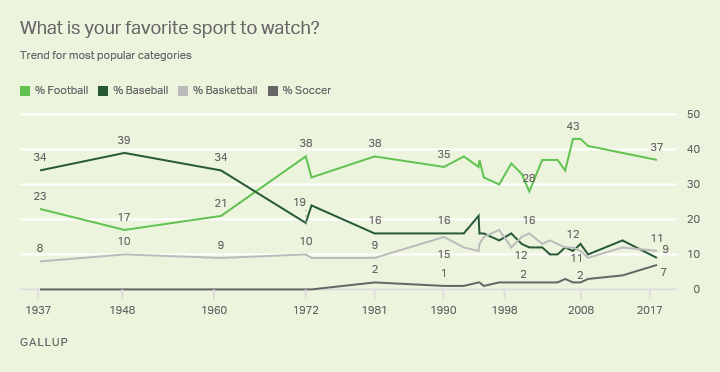
\includegraphics[width=0.75\textwidth]{Gallupfavoritesport.png}
\end{center}
\caption{Gallup polling data on the topic of the favorite sports 
  of Americans over time.}
\label{Gallup}
\end{figure}


These weights are obtained from survey data from the US because similar data 
is unavailable from other countries.
%only.  We did this because rich survey data on the topic of interest in 
%baseball is unavailable from the other countries.  
We applied these same 
weights to all of the other countries, even though interest in baseball in 
these other countries is thought to either be on par with or much greater 
than the US.  Therefore our weighting regimes address, and in fact, 
overcompensate for any potential shortcomings of no weighting.

The weights are now added to our analysis, and we construct four new datasets 
with reweighted populations corresponding to each of the four weighting 
schemes outlined in Table 4.


\begin{knitrout}
\definecolor{shadecolor}{rgb}{0.969, 0.969, 0.969}\color{fgcolor}\begin{kframe}
\begin{alltt}
\hlcom{# compute w1 based on information from }
\hlcom{# Gallup on baseball fans (50% fans before 1940)}
\hlstd{w1} \hlkwb{<-} \hlkwd{c}\hlstd{(}\hlkwd{rep}\hlstd{(}\hlnum{0.5}\hlstd{,} \hlnum{6}\hlstd{),} \hlkwd{rep}\hlstd{(}\hlnum{0.4}\hlstd{,} \hlnum{9}\hlstd{))}

\hlcom{# construct rewighted dataset with respect to w1}
\hlstd{data.w1} \hlkwb{<-} \hlstd{data}
\hlstd{data.w1[,} \hlnum{2}\hlstd{]} \hlkwb{<-} \hlstd{data.w1[,} \hlnum{2}\hlstd{]} \hlopt{*} \hlstd{w1}
\hlstd{data.w1[,} \hlnum{3}\hlstd{]} \hlkwb{<-} \hlkwd{cumsum}\hlstd{(data.w1[,} \hlnum{2}\hlstd{])} \hlopt{/} \hlkwd{sum}\hlstd{(data.w1[,} \hlnum{2}\hlstd{])}

\hlcom{# compute w2 based on information from }
\hlcom{# Gallup on baseball fans (60% fans before 1940)}
\hlstd{w2} \hlkwb{<-} \hlkwd{c}\hlstd{(}\hlkwd{rep}\hlstd{(}\hlnum{0.6}\hlstd{,} \hlnum{6}\hlstd{),} \hlkwd{rep}\hlstd{(}\hlnum{0.4}\hlstd{,} \hlnum{9}\hlstd{))}

\hlcom{# construct rewighted dataset with respect to w2}
\hlstd{data.w2} \hlkwb{<-} \hlstd{data}
\hlstd{data.w2[,} \hlnum{2}\hlstd{]} \hlkwb{<-} \hlstd{data.w2[,} \hlnum{2}\hlstd{]} \hlopt{*} \hlstd{w2}
\hlstd{data.w2[,} \hlnum{3}\hlstd{]} \hlkwb{<-} \hlkwd{cumsum}\hlstd{(data.w2[,} \hlnum{2}\hlstd{])} \hlopt{/} \hlkwd{sum}\hlstd{(data.w2[,} \hlnum{2}\hlstd{])}

\hlcom{# compute w3 based on information from }
\hlcom{# Gallup on favorite sport}
\hlstd{w3} \hlkwb{<-} \hlkwd{c}\hlstd{(}\hlkwd{rep}\hlstd{(}\hlnum{0.4}\hlstd{,} \hlnum{6}\hlstd{),} \hlnum{0.35}\hlstd{,} \hlnum{0.38}\hlstd{,} \hlnum{0.34}\hlstd{,} \hlnum{0.28}\hlstd{,} \hlnum{0.16}\hlstd{,} \hlnum{0.16}\hlstd{,} \hlnum{0.13}\hlstd{,} \hlnum{0.12}\hlstd{,} \hlnum{0.10}\hlstd{)}

\hlcom{# construct rewighted dataset with respect to w3}
\hlstd{data.w3} \hlkwb{<-} \hlstd{data}
\hlstd{data.w3[,} \hlnum{2}\hlstd{]} \hlkwb{<-} \hlstd{data.w3[,} \hlnum{2}\hlstd{]} \hlopt{*} \hlstd{w3}
\hlstd{data.w3[,} \hlnum{3}\hlstd{]} \hlkwb{<-} \hlkwd{cumsum}\hlstd{(data.w3[,} \hlnum{2}\hlstd{])} \hlopt{/} \hlkwd{sum}\hlstd{(data.w3[,} \hlnum{2}\hlstd{])}

\hlcom{# construct rewighted dataset with respect to w4}
\hlstd{w4} \hlkwb{<-} \hlstd{(w2} \hlopt{+} \hlstd{w3)} \hlopt{/} \hlnum{2}
\hlstd{data.w4} \hlkwb{<-} \hlstd{data}
\hlstd{data.w4[,} \hlnum{2}\hlstd{]} \hlkwb{<-} \hlstd{data.w4[,} \hlnum{2}\hlstd{]} \hlopt{*} \hlstd{w4}
\hlstd{data.w4[,} \hlnum{3}\hlstd{]} \hlkwb{<-} \hlkwd{cumsum}\hlstd{(data.w4[,} \hlnum{2}\hlstd{])} \hlopt{/} \hlkwd{sum}\hlstd{(data.w4[,} \hlnum{2}\hlstd{])}
\end{alltt}
\end{kframe}
\end{knitrout}

Table 4 displays the weighting regimes used in our analysis, and it is 
constructed with the code below.

\begin{kframe}
\begin{alltt}
\hlstd{tab} \hlkwb{<-} \hlkwd{cbind}\hlstd{(w1,w2,w3,w4)}
\hlkwd{rownames}\hlstd{(tab)} \hlkwb{<-} \hlstd{year}
\hlkwd{print}\hlstd{(}\hlkwd{xtable}\hlstd{(}\hlkwd{t}\hlstd{(tab),} \hlcom{#digits = c(0,0,2,2,2,2), }
  \hlkwc{digits} \hlstd{=} \hlkwd{cbind}\hlstd{(}\hlkwd{rep}\hlstd{(}\hlnum{0}\hlstd{,} \hlnum{4}\hlstd{),} \hlkwd{matrix}\hlstd{(}\hlnum{2}\hlstd{,} \hlkwc{ncol} \hlstd{=} \hlnum{15}\hlstd{,} \hlkwc{nrow} \hlstd{=} \hlnum{4}\hlstd{)),}
  \hlkwc{caption} \hlstd{=} \hlstr{"Weighting regimes"}\hlstd{),} \hlkwc{size} \hlstd{=} \hlstr{"footnotesize"}\hlstd{,}
  \hlcom{#hline.after = c(-1,0,nrow(data)))}
  \hlkwc{hline.after} \hlstd{=} \hlkwd{c}\hlstd{(}\hlopt{-}\hlnum{1}\hlstd{,}\hlnum{0}\hlstd{,}\hlnum{4}\hlstd{))}
\end{alltt}
\end{kframe}% latex table generated in R 3.4.4 by xtable 1.8-3 package
% Sun Aug 18 17:10:30 2019
\begin{table}[ht]
\centering
\begingroup\footnotesize
\begin{tabular}{rrrrrrrrrrrrrrrr}
  \hline
 & 1880 & 1890 & 1900 & 1910 & 1920 & 1930 & 1940 & 1950 & 1960 & 1970 & 1980 & 1990 & 2000 & 2010 & 2015 \\ 
  \hline
w1 & 0.50 & 0.50 & 0.50 & 0.50 & 0.50 & 0.50 & 0.40 & 0.40 & 0.40 & 0.40 & 0.40 & 0.40 & 0.40 & 0.40 & 0.40 \\ 
  w2 & 0.60 & 0.60 & 0.60 & 0.60 & 0.60 & 0.60 & 0.40 & 0.40 & 0.40 & 0.40 & 0.40 & 0.40 & 0.40 & 0.40 & 0.40 \\ 
  w3 & 0.40 & 0.40 & 0.40 & 0.40 & 0.40 & 0.40 & 0.35 & 0.38 & 0.34 & 0.28 & 0.16 & 0.16 & 0.13 & 0.12 & 0.10 \\ 
  w4 & 0.50 & 0.50 & 0.50 & 0.50 & 0.50 & 0.50 & 0.38 & 0.39 & 0.37 & 0.34 & 0.28 & 0.28 & 0.27 & 0.26 & 0.25 \\ 
   \hline
\end{tabular}
\endgroup
\caption{Weighting regimes} 
\end{table}



Table~\ref{probvalues.weights} shows the effect of these weighting regimes as 
applied to the results in Table~\ref{probvalues}.  
%The results of weighting populations and then recalculating 
%the probabilities and chances displayed in  
%are displayed in .  
The conclusions from weighting populations with respect to w1, w2, and w4 in 
Table~\ref{probvalues.weights} are largely consistent with those in 
Table~\ref{probvalues}.  %It is very unlikely that such a sparsely populated 
%time period could have produced so many historically great baseball players.  
The third weighting regime presents some conflicting conclusions.  When 
weighting populations with respect to w3 we see that popular opinion and 
bWAR overrepresent players who started their careers before 1950.  
However, the same is not so for fWAR and ESPN. 
The overall finding of this sensitivity analysis is that conservatively 
weighting populations with respect to fan interest in baseball yields the 
conclusion as the analysis in Section 4:
it is very unlikely that the pre-1950s time period could 
have produced so many historically great baseball players.  

We now perform the same Binomial distribution calculations in the previous 
Section with respect to the reweighted populations and each top 10 and top 25 
list depicted in Table~\ref{top25}. %are conducted using R statistical 
%software below.  The results are provided in Table~\ref{probvalues}. 



\begin{knitrout}
\definecolor{shadecolor}{rgb}{0.969, 0.969, 0.969}\color{fgcolor}\begin{kframe}
\begin{alltt}
\hlcom{## Recompute extreme probabilities consistent with w1}
\hlstd{p.w1} \hlkwb{<-} \hlstd{data.w1[}\hlnum{8}\hlstd{,} \hlnum{3}\hlstd{]}
\hlstd{pranker10.w1} \hlkwb{<-} \hlkwd{pbinom}\hlstd{(ranker10} \hlopt{-} \hlnum{1}\hlstd{,} \hlkwc{p} \hlstd{= p.w1,} \hlkwc{size} \hlstd{=} \hlnum{10}\hlstd{,} \hlkwc{lower} \hlstd{=} \hlnum{FALSE}\hlstd{)}
\hlstd{pbWAR10.w1}   \hlkwb{<-} \hlkwd{pbinom}\hlstd{(bWAR10} \hlopt{-} \hlnum{1}\hlstd{,} \hlkwc{p} \hlstd{= p.w1,} \hlkwc{size} \hlstd{=} \hlnum{10}\hlstd{,} \hlkwc{lower} \hlstd{=} \hlnum{FALSE}\hlstd{)}
\hlstd{pfWAR10.w1}   \hlkwb{<-} \hlkwd{pbinom}\hlstd{(fWAR10} \hlopt{-} \hlnum{1}\hlstd{,} \hlkwc{p} \hlstd{= p.w1,} \hlkwc{size} \hlstd{=} \hlnum{10}\hlstd{,} \hlkwc{lower} \hlstd{=} \hlnum{FALSE}\hlstd{)}
\hlstd{pESPN10.w1}   \hlkwb{<-} \hlkwd{pbinom}\hlstd{(ESPN10} \hlopt{-} \hlnum{1}\hlstd{,} \hlkwc{p} \hlstd{= p.w1,} \hlkwc{size} \hlstd{=} \hlnum{10}\hlstd{,} \hlkwc{lower} \hlstd{=} \hlnum{FALSE}\hlstd{)}
\hlstd{pranker25.w1} \hlkwb{<-} \hlkwd{pbinom}\hlstd{(ranker25} \hlopt{-} \hlnum{1}\hlstd{,} \hlkwc{p} \hlstd{= p.w1,} \hlkwc{size} \hlstd{=} \hlnum{25}\hlstd{,} \hlkwc{lower} \hlstd{=} \hlnum{FALSE}\hlstd{)}
\hlstd{pbWAR25.w1}   \hlkwb{<-} \hlkwd{pbinom}\hlstd{(bWAR25} \hlopt{-} \hlnum{1}\hlstd{,} \hlkwc{p} \hlstd{= p.w1,} \hlkwc{size} \hlstd{=} \hlnum{25}\hlstd{,} \hlkwc{lower} \hlstd{=} \hlnum{FALSE}\hlstd{)}
\hlstd{pfWAR25.w1}   \hlkwb{<-} \hlkwd{pbinom}\hlstd{(fWAR25} \hlopt{-} \hlnum{1}\hlstd{,} \hlkwc{p} \hlstd{= p.w1,} \hlkwc{size} \hlstd{=} \hlnum{25}\hlstd{,} \hlkwc{lower} \hlstd{=} \hlnum{FALSE}\hlstd{)}
\hlstd{pESPN25.w1}   \hlkwb{<-} \hlkwd{pbinom}\hlstd{(ESPN25} \hlopt{-} \hlnum{1}\hlstd{,} \hlkwc{p} \hlstd{= p.w1,} \hlkwc{size} \hlstd{=} \hlnum{25}\hlstd{,} \hlkwc{lower} \hlstd{=} \hlnum{FALSE}\hlstd{)}

\hlcom{## Recompute extreme probabilities consistent with w2}
\hlstd{p.w2} \hlkwb{<-} \hlstd{data.w2[}\hlnum{8}\hlstd{,} \hlnum{3}\hlstd{]}
\hlstd{pranker10.w2} \hlkwb{<-} \hlkwd{pbinom}\hlstd{(ranker10} \hlopt{-} \hlnum{1}\hlstd{,} \hlkwc{p} \hlstd{= p.w2,} \hlkwc{size} \hlstd{=} \hlnum{10}\hlstd{,} \hlkwc{lower} \hlstd{=} \hlnum{FALSE}\hlstd{)}
\hlstd{pbWAR10.w2}   \hlkwb{<-} \hlkwd{pbinom}\hlstd{(bWAR10} \hlopt{-} \hlnum{1}\hlstd{,} \hlkwc{p} \hlstd{= p.w2,} \hlkwc{size} \hlstd{=} \hlnum{10}\hlstd{,} \hlkwc{lower} \hlstd{=} \hlnum{FALSE}\hlstd{)}
\hlstd{pfWAR10.w2}   \hlkwb{<-} \hlkwd{pbinom}\hlstd{(fWAR10} \hlopt{-} \hlnum{1}\hlstd{,} \hlkwc{p} \hlstd{= p.w2,} \hlkwc{size} \hlstd{=} \hlnum{10}\hlstd{,} \hlkwc{lower} \hlstd{=} \hlnum{FALSE}\hlstd{)}
\hlstd{pESPN10.w2}   \hlkwb{<-} \hlkwd{pbinom}\hlstd{(ESPN10} \hlopt{-} \hlnum{1}\hlstd{,} \hlkwc{p} \hlstd{= p.w2,} \hlkwc{size} \hlstd{=} \hlnum{10}\hlstd{,} \hlkwc{lower} \hlstd{=} \hlnum{FALSE}\hlstd{)}
\hlstd{pranker25.w2} \hlkwb{<-} \hlkwd{pbinom}\hlstd{(ranker25} \hlopt{-} \hlnum{1}\hlstd{,} \hlkwc{p} \hlstd{= p.w2,} \hlkwc{size} \hlstd{=} \hlnum{25}\hlstd{,} \hlkwc{lower} \hlstd{=} \hlnum{FALSE}\hlstd{)}
\hlstd{pbWAR25.w2}   \hlkwb{<-} \hlkwd{pbinom}\hlstd{(bWAR25} \hlopt{-} \hlnum{1}\hlstd{,} \hlkwc{p} \hlstd{= p.w2,} \hlkwc{size} \hlstd{=} \hlnum{25}\hlstd{,} \hlkwc{lower} \hlstd{=} \hlnum{FALSE}\hlstd{)}
\hlstd{pfWAR25.w2}   \hlkwb{<-} \hlkwd{pbinom}\hlstd{(fWAR25} \hlopt{-} \hlnum{1}\hlstd{,} \hlkwc{p} \hlstd{= p.w2,} \hlkwc{size} \hlstd{=} \hlnum{25}\hlstd{,} \hlkwc{lower} \hlstd{=} \hlnum{FALSE}\hlstd{)}
\hlstd{pESPN25.w2}   \hlkwb{<-} \hlkwd{pbinom}\hlstd{(ESPN25} \hlopt{-} \hlnum{1}\hlstd{,} \hlkwc{p} \hlstd{= p.w2,} \hlkwc{size} \hlstd{=} \hlnum{25}\hlstd{,} \hlkwc{lower} \hlstd{=} \hlnum{FALSE}\hlstd{)}

\hlcom{## Recompute extreme probabilities consistent with w3}
\hlstd{p.w3} \hlkwb{<-} \hlstd{data.w3[}\hlnum{8}\hlstd{,} \hlnum{3}\hlstd{]}
\hlstd{pranker10.w3} \hlkwb{<-} \hlkwd{pbinom}\hlstd{(ranker10} \hlopt{-} \hlnum{1}\hlstd{,} \hlkwc{p} \hlstd{= p.w3,} \hlkwc{size} \hlstd{=} \hlnum{10}\hlstd{,} \hlkwc{lower} \hlstd{=} \hlnum{FALSE}\hlstd{)}
\hlstd{pbWAR10.w3}   \hlkwb{<-} \hlkwd{pbinom}\hlstd{(bWAR10} \hlopt{-} \hlnum{1}\hlstd{,} \hlkwc{p} \hlstd{= p.w3,} \hlkwc{size} \hlstd{=} \hlnum{10}\hlstd{,} \hlkwc{lower} \hlstd{=} \hlnum{FALSE}\hlstd{)}
\hlstd{pfWAR10.w3}   \hlkwb{<-} \hlkwd{pbinom}\hlstd{(fWAR10} \hlopt{-} \hlnum{1}\hlstd{,} \hlkwc{p} \hlstd{= p.w3,} \hlkwc{size} \hlstd{=} \hlnum{10}\hlstd{,} \hlkwc{lower} \hlstd{=} \hlnum{FALSE}\hlstd{)}
\hlstd{pESPN10.w3}   \hlkwb{<-} \hlkwd{pbinom}\hlstd{(ESPN10} \hlopt{-} \hlnum{1}\hlstd{,} \hlkwc{p} \hlstd{= p.w3,} \hlkwc{size} \hlstd{=} \hlnum{10}\hlstd{,} \hlkwc{lower} \hlstd{=} \hlnum{FALSE}\hlstd{)}
\hlstd{pranker25.w3} \hlkwb{<-} \hlkwd{pbinom}\hlstd{(ranker25} \hlopt{-} \hlnum{1}\hlstd{,} \hlkwc{p} \hlstd{= p.w3,} \hlkwc{size} \hlstd{=} \hlnum{25}\hlstd{,} \hlkwc{lower} \hlstd{=} \hlnum{FALSE}\hlstd{)}
\hlstd{pbWAR25.w3}   \hlkwb{<-} \hlkwd{pbinom}\hlstd{(bWAR25} \hlopt{-} \hlnum{1}\hlstd{,} \hlkwc{p} \hlstd{= p.w3,} \hlkwc{size} \hlstd{=} \hlnum{25}\hlstd{,} \hlkwc{lower} \hlstd{=} \hlnum{FALSE}\hlstd{)}
\hlstd{pfWAR25.w3}   \hlkwb{<-} \hlkwd{pbinom}\hlstd{(fWAR25} \hlopt{-} \hlnum{1}\hlstd{,} \hlkwc{p} \hlstd{= p.w3,} \hlkwc{size} \hlstd{=} \hlnum{25}\hlstd{,} \hlkwc{lower} \hlstd{=} \hlnum{FALSE}\hlstd{)}
\hlstd{pESPN25.w3}   \hlkwb{<-} \hlkwd{pbinom}\hlstd{(ESPN25} \hlopt{-} \hlnum{1}\hlstd{,} \hlkwc{p} \hlstd{= p.w3,} \hlkwc{size} \hlstd{=} \hlnum{25}\hlstd{,} \hlkwc{lower} \hlstd{=} \hlnum{FALSE}\hlstd{)}

\hlcom{## Recompute extreme probabilities consistent with w4}
\hlstd{p.w4} \hlkwb{<-} \hlstd{data.w4[}\hlnum{8}\hlstd{,} \hlnum{3}\hlstd{]}
\hlstd{pranker10.w4} \hlkwb{<-} \hlkwd{pbinom}\hlstd{(ranker10} \hlopt{-} \hlnum{1}\hlstd{,} \hlkwc{p} \hlstd{= p.w4,} \hlkwc{size} \hlstd{=} \hlnum{10}\hlstd{,} \hlkwc{lower} \hlstd{=} \hlnum{FALSE}\hlstd{)}
\hlstd{pbWAR10.w4}   \hlkwb{<-} \hlkwd{pbinom}\hlstd{(bWAR10} \hlopt{-} \hlnum{1}\hlstd{,} \hlkwc{p} \hlstd{= p.w4,} \hlkwc{size} \hlstd{=} \hlnum{10}\hlstd{,} \hlkwc{lower} \hlstd{=} \hlnum{FALSE}\hlstd{)}
\hlstd{pfWAR10.w4}   \hlkwb{<-} \hlkwd{pbinom}\hlstd{(fWAR10} \hlopt{-} \hlnum{1}\hlstd{,} \hlkwc{p} \hlstd{= p.w4,} \hlkwc{size} \hlstd{=} \hlnum{10}\hlstd{,} \hlkwc{lower} \hlstd{=} \hlnum{FALSE}\hlstd{)}
\hlstd{pESPN10.w4}   \hlkwb{<-} \hlkwd{pbinom}\hlstd{(ESPN10} \hlopt{-} \hlnum{1}\hlstd{,} \hlkwc{p} \hlstd{= p.w4,} \hlkwc{size} \hlstd{=} \hlnum{10}\hlstd{,} \hlkwc{lower} \hlstd{=} \hlnum{FALSE}\hlstd{)}
\hlstd{pranker25.w4} \hlkwb{<-} \hlkwd{pbinom}\hlstd{(ranker25} \hlopt{-} \hlnum{1}\hlstd{,} \hlkwc{p} \hlstd{= p.w4,} \hlkwc{size} \hlstd{=} \hlnum{25}\hlstd{,} \hlkwc{lower} \hlstd{=} \hlnum{FALSE}\hlstd{)}
\hlstd{pbWAR25.w4}   \hlkwb{<-} \hlkwd{pbinom}\hlstd{(bWAR25} \hlopt{-} \hlnum{1}\hlstd{,} \hlkwc{p} \hlstd{= p.w4,} \hlkwc{size} \hlstd{=} \hlnum{25}\hlstd{,} \hlkwc{lower} \hlstd{=} \hlnum{FALSE}\hlstd{)}
\hlstd{pfWAR25.w4}   \hlkwb{<-} \hlkwd{pbinom}\hlstd{(fWAR25} \hlopt{-} \hlnum{1}\hlstd{,} \hlkwc{p} \hlstd{= p.w4,} \hlkwc{size} \hlstd{=} \hlnum{25}\hlstd{,} \hlkwc{lower} \hlstd{=} \hlnum{FALSE}\hlstd{)}
\hlstd{pESPN25.w4}   \hlkwb{<-} \hlkwd{pbinom}\hlstd{(ESPN25} \hlopt{-} \hlnum{1}\hlstd{,} \hlkwc{p} \hlstd{= p.w4,} \hlkwc{size} \hlstd{=} \hlnum{25}\hlstd{,} \hlkwc{lower} \hlstd{=} \hlnum{FALSE}\hlstd{)}
\end{alltt}
\end{kframe}
\end{knitrout}





\begin{table}[h!]
\begin{center}
\begin{tabular}{llllll}
\hline
 weight & &  Ranker  &  bWAR  &  fWAR  &  ESPN \\
 \hline
w1 & probability of extreme event in top 10 list 
  & 0.00122 
  & 0.0084 
  & 0.0084 
  & 0.0407 \\
& probability of extreme event in top 25 list 
  & \ensuremath{2.68\times 10^{-5}} 
  & \ensuremath{2.68\times 10^{-5}} 
  & 0.0025 
  & 0.00847 \\
& chance of extreme event in top 10 list 
  & 1 in 823 
  & 1 in 119 
  & 1 in 119 
  & 1 in 25 \\
& chance of extreme event in top 25 list 
  & 1 in \ensuremath{3.7371\times 10^{4}} 
  & 1 in \ensuremath{3.7371\times 10^{4}} 
  & 1 in 400 
  & 1 in 118 \\
  & & & & & \\
w2 & probability of extreme event in top 10 list 
  & 0.00231 
  & 0.0141 
  & 0.0141 
  & 0.0605 \\
& probability of extreme event in top 25 list 
  & \ensuremath{9.47\times 10^{-5}} 
  & \ensuremath{9.47\times 10^{-5}} 
  & 0.0061 
  & 0.0183 \\
& chance of extreme event in top 10 list 
  & 1 in 434 
  & 1 in 71 
  & 1 in 71 
  & 1 in 17 \\
& chance of extreme event in top 25 list 
  & 1 in \ensuremath{1.0557\times 10^{4}} 
  & 1 in \ensuremath{1.0557\times 10^{4}} 
  & 1 in 164 
  & 1 in 55 \\
  & & & & & \\
w3 & probability of extreme event in top 10 list 
  & 0.0311 
  & 0.109 
  & 0.109 
  & 0.274 \\
& probability of extreme event in top 25 list 
  & 0.0128 
  & 0.0128 
  & 0.152 
  & 0.267 \\
& chance of extreme event in top 10 list 
  & 1 in 32 
  & 1 in 9 
  & 1 in 9 
  & 1 in 3.7 \\
& chance of extreme event in top 25 list 
  & 1 in 78 
  & 1 in 78 
  & 1 in 6.6 
  & 1 in 3.8 \\
  & & & & & \\  
w4 & probability of extreme event in top 10 list 
  & 0.00623 
  & 0.0312 
  & 0.0312 
  & 0.11 \\
& probability of extreme event in top 25 list 
  & \ensuremath{6.5\times 10^{-4}} 
  & \ensuremath{6.5\times 10^{-4}} 
  & 0.0228 
  & 0.0561 \\
& chance of extreme event in top 10 list 
  & 1 in 160 
  & 1 in 32 
  & 1 in 32 
  & 1 in 9.1 \\
& chance of extreme event in top 25 list 
  & 1 in 1537 
  & 1 in 1537 
  & 1 in 44 
  & 1 in 18 \\
  \hline
\end{tabular}
\end{center}
\caption{The probability and chance (1 in 1/probability, rounded) 
  of each extreme event calculation corresponding to the four lists in 
  Table~\ref{top25} after the MLB eligible population in Table 1 is 
  weighted according to the four conservative weighting regimes.}
\label{probvalues.weights}
\end{table}



\section{Additional comparison methods}

%In the previous Sections we observe that popular opinion (i.e., nostalgia) 
%and performance metrics are in conflict with the population dynamics that 
%underlie the distribution of the eligible MLB talent pool.  
%%%Our evaluation metric model free analysis of great players conflicts with the 
%%%top 25 list in Table~\ref{top25}, conventional evaluation metrics such as Wins 
%%%Above Replacement (WAR), and a more sophisticated era-adjusted detrending 
%%%metric of PPS. The underlying principles of these competing metrics are now 
%%%compared with out methodology. We start with WAR.
%We now critique additional methods that compare players across eras.  



\subsection{Versus your peers methods}
\label{WARcritique}

There are several methods which are used to compare players across eras that 
do so by computing a baseline achievement threshold within one season and then 
comparing players to that baseline.  These methods then rank players by how far 
they stood above their peers, the greatest players were better than their peers 
by the largest amount. 
%As noted in the Introduction, examples include 
%bWAR, 
%fWAR, 
%adjusted OPS+,
%adjusted ERA+,
%and computing normal scores.
%This manner of player comparison is purely statistical and it ignores talent 
%discrepancies that exist across seasons.  
We have shown that this approach can exhibit major biases in player comparisons 
as evidenced by career bWAR and fWAR.  Adjusted OPS+ is a worse offender 
than bWAR or fWAR.  Adjusted ERA+ is right in line with ESPN rankings.

%Philosophically speaking, WAR is a one-number summary of the added value of a 
%player over a ``replacement" level player. It is a statistic but it is not 
%thought about as a statistic in the way statisticians think about statistics. 
%For instance, the replacement level player, which is central to the 
%interpretation of WAR, is not a fixed and known entity but rather a random 
%outcome. In each year, the perceived value of the replacement player changes 
%based on the individuals comprising the statistical outcome of that year's 
%baseball season. Therefore, the most central component to the calculation of 
%WAR is both random and is subject to a strong era-effect. The ESPN top 25 list 
%used a variation of WAR to compare players \citep*{szymborski}. Another 
%disadvantage of WAR is that it is more of a philosophical concept than a 
%calculable statistic. There are many different ways to calculate WAR 
%\citep*{bref, fangraphs} and these differing calculations assign different 
%values to the same performance. The arbitrariness of WAR as an actual 
%statistical tool coupled with its inherent randomness makes it a blunt tool 
%for comparing performances across eras. As an example of this, consider the 
%defensive comparison between Ozzie Smith's 1983 season and Rogers Hornsby's 
%1917 season provided in Table~\ref{Rajah}. Clearly Ozzie Smith had the 
%superior defensive season but Rogers Hornsby's defensive WAR is substantially 
%higher. In all, we see that it does not make sense to use WAR as a way to 
%compare players across eras.


%\begin{table}[h!]
%\begin{center}
%\begin{tabular}{l|cccccc}
%& pos & Fld\% & Chances & Errors & RF/9 & dWAR \\
%\hline
%Rogers Hornsby & SS & 0.939 & 847 & 52 & 5.62 & 3.5 \\
%Ozzie Smith    & SS & 0.975 & 844 & 21 & 5.51 & 2.3 \\
%\hline
%\end{tabular}
%\end{center}
%\caption{Comparison of Rogers Hornsby's 1917 defensive season and 
%  Ozzie Smith's 1983 defensive season.}
%\label{Rajah}
%\end{table}


\subsection{PPS detrending}

We describe and critique the methodology of \citet{petersen} (PPS). 
%in the context of comparing players across eras.  
%We will refer to their paper as PPS due to repeated mentions.  
As described in PPS, they detrend player statistics by normalizing 
achievements to seasonal averages, which they claim accounts for changes in 
relative player ability resulting from both exogenous and endogenous factors, 
such as 
talent dilution from expansion, 
equipment and training improvements, 
as well as performance enhancing drug usage. 
PPS misunderstands the effect of talent dilution from expansion and ignores 
reality.  The talent pool was more diluted in the earlier eras of 
baseball than now because of a small relative eligible population size and 
the exclusion of entire populations of people on racial grounds.  
See Table~\ref{dilution} for the specifics.  PPS's position with respect 
to equipment and training improvements is likewise not without fault 
because the same improvements are equally available to every competitor.  
%PPS also does not account for the effect of modern day filming as a way to 
%gain insight on opponents' strengths and weakness in their training 
%improvements assumption.  
Finally, PPS does not account for increases in salary compensation enjoyed by 
MLB players in modern eras, and their methodology fails to address 
segregation prior to 1947.


\begin{table}[h!]
\begin{center}
\begin{tabular}{lcccc}
\hline
year & eligible pop. & number of teams & roster size & eligible pop. per roster spot \\
\hline
1880 & 4.44  & 8  & 15 & 37   \\
1890 & 5.01  & 8  & 15 & 41.7   \\
1900 & 5.58  & 8  & 15 & 46.5   \\
1910 & 8.55  & 16 & 25 & 21.4  \\
1920 & 8.93  & 16 & 25 & 22.3  \\
  & & & &  \\
1930 & 9.92  & 16 & 25 & 24.8  \\
1940 & 11.13  & 16 & 25 & 27.8  \\
1950 & 11.59  & 16 & 25 & 29  \\
1960 & 18.42  & 16 & 25 & 46.1  \\
1970 & 24.49  & 24 & 25 & 40.8  \\
  & & & &  \\
1980 & 33.93 & 26 & 25 & 52.2 \\
1990 & 37.46 & 26 & 25 & 57.6 \\
2000 & 60.6 & 30 & 25 & 80.8 \\
2010 & 72.21 & 30 & 25 & 96.3 \\
\hline
\end{tabular}
\end{center}
\caption{Relative talent dilution when considering the MLB eligible population 
  sizes at select time periods. Eligible population totals are in millions in 
  column 2 and are in thousands in column 5. }
\label{dilution}
\end{table}



The mathematics of PPS detrending is also questionable in the context of 
comparing baseball players across eras. 
PPS notes that the evolutionary nature of competition results in a 
non-stationary rate of success.  They then detrend player 
statistics by normalizing achievements to seasonal averages.  
The normalization goes as follows: 
  Suppose a player hits 40 homeruns in a given season and that the league 
  average prowess for homerun hitting in that season is 10 homeruns. If the 
  historical average prowess for homerun hitting is 5 homeruns then our 
  player's detrended homerun count in that particular season is 
  $40\times(5/10) = 20$.  In general, the detrending formula is 
  $Y \times (\text{historic prowess} / \text{league prowess})$ where $Y$ is 
  individual prowess for a particular player in a given season.
%Fundamentally different approaches for detrending are advocated in 
%authoritative textbooks such as 
% Introduction to Time Series and Forecasting,
%   by
% Peter J. Brockwell and Richard A. Davis,
% Time Series Analysis and Its Applications With R Examples, 
%   by 
%   Robert H. Shumway and David S. Stoffer, 
% and
% Time Series Analysis and Forecasting by Example, 
%   by
%   S{\o}ren Bisgaard and Murat Kulahci. %,
%%%and all of the authors conversations with statisticians.  
%%%None of which involve the 
%%%incorporation of an implicitly volatile quantity. 
%The supposition that $x_i^D(t)$ offers an objective comparison of players 
%across time is questionable for reasons previously mentioned.  
%The average $\overline{P}$ treats all eras as equals in its computation. 
%Different eras should be given different weights reflecting richness of 
%the available talent pool. Here are some facts suggesting that the talent 
% pool has changed over time. In 1920, the average MLB salary was \$5000 
%(\$60,000 in 2015 dollars). In 2015, the average salary is \$4 million. 
%Before 1947, African-American ball players were excluded from participation 
%in MLB games. Many MLB players and/or potential MLB players served in the 
%armed forces during WWII, the Korean War, the Vietnam War, and the 
%Gulf Wars.  The metric $x_i^D(t)$ takes none of these factors into 
%additional consideration. 
%%%In addition, there is no consensus on how old-time players would perform 
%%%with modern training at the disposal to themselves and their competition 
%%%as a whole. 
%Instead of the detrended metric \eqref{detrended}, one could just as easily 
%construct the detrended metric 
%\begin{equation} \label{inverse}
%  x_i^{D^{\prime}}(t) = x_i(t)\frac{\langle P(t) \rangle}{\overline{P}}. 
%\end{equation}
%which also maintains the merits of dimensionlessness and detrending as they 
%state it. However, the metric \eqref{inverse} reaches the exact opposite 
%conclusions as the metric \eqref{detrended}. The formulation of 
%$x_i^{D^{\prime}}(t)$ rewards prowess from strong eras and punishes prowess 
%from weak eras.  The only difference between the formulations of the two 
%detrending metrics is the placement of $\langle P(t) \rangle$ relative to 
%$\overline{P}$.  The mathematical formulation of PPS detrending is an 
%artifact of the assumptions made.  Detrending using \eqref{inverse} maintains 
%all of the merits of PPS detrending but reaches opposite conclusions with the 
%justification of having the opposite opinion as the authors of PPS.
We see PPS detrending as an inflationary metric of relative prowesses 
and not a detrending metric.  
Fundamentally different approaches for detrending are advocated in 
authoritative textbooks such as 
 Introduction to Time Series and Forecasting,
   by
 Peter J. Brockwell and Richard A. Davis.
%We agree with Petersen when he says, 
%``detrending corresponds to removing the inflationary factor, so we could 
%compare two items like the cost of a candy bar in 1920 to the cost of a 
%candy bar in 2000.  In this case, we compare Babe Ruth's home runs--the 
%ability of someone to get a home run then versus now--and you see Babe 
%Ruth actually hit a lot of home runs on this relative basis,'' 
%in a BU Today piece written by Rachel Johnson.
%\citep{johnson2011petersen}.  
Table 2 in PPS displays the top 25 career detrended homerun totals.  Their 
top 10 list contains 7 players who started their careers before 1950 
(the same as Ranker), and their 
top 25 list contains 12 players who started their careers before 1950 
(the same as fWAR).
It is clear that having higher prowess relative to your peers, hitting more 
runs in this case, is not indicative of a player's prowess with respect to 
peers from fundamentally different eras.  
%Additionally, PPS's methodology does not account for segregation of baseball 
%prior to 1947.  There is minimal support for Petersen's claim that PPS detrending 
%makes the statistics fairer which appears in Johnson's article.




%\vspace{1cm}\noindent {\bf Side quotes}: \\

%That is, according to passionate baseball fan Alexander Petersen.  Using 
%statistical physics theory, he's found a way to compare baseball players over 
%the generations, whether they played in the dead-ball era in the early 1900s 
%or the steroids era beginning in the 1990s \citep{johnson2011petersen}. \\

%``Basically,'' says Petersen, ``detrending corresponds to removing the 
%inflationary factor, so we could compare two items like the cost of a candy 
%bar in 1920 to the cost of a candy bar in 2000. In this case, we compare Babe 
%Ruth's home runs--the ability of someone to get a home run then versus 
%now--and you see Babe Ruth actually hit a lot of home runs on this relative 
%basis.'' Petersen's new statistics compare career longevity, success, and 
%productivity. When comparing the baseball statistics, he was startled to 
%discover a statistical pattern, what he calls a beautiful power-law curve 
%(a type of bell curve), emerging from seemingly random careers 
%\citep{johnson2011petersen}. \\


%``The relative significance of their accomplishments gets reduced because 
%their contemporaries are hitting a lot of home runs as well,'' says 
%Petersen. Players like Babe Ruth, Lou Gehrig, and Ted Williams shoot up the 
%list because they were giants in their own era as well as across the 
%decades.  Petersen says his approach is a way to make the statistics fairer: 
%besides accounting for the possible effects of steroids, detrending allows 
%for changes in equipment, diet, conditioning, even medical procedures like 
%Tommy John surgery (replacing a ligament in the elbow with a tendon to 
%lengthen a pitching career), all of which have changed the game since 
%Ruth's time \citep{johnson2011petersen}. \\



\subsection{Era bridging}

\citet{berry1999eras} claim that their era bridging technique accounts for 
talent discrepancies across eras.  However, they do not explicitly 
parameterize this in their hierarchical models.  They state that 
``globalization has been less pronounced in the MLB (relative to other 
sports)... Baseball has remained fairly stable within the 
United States, where it has been an important part of the culture for more 
than a century'' \citep{berry1999eras}.  This rationale ignores 
segregation, increases in the MLB eligible population 
relative to available roster spots, and increases in the average overall 
talent of that population.  %They claim that they capture the 
%changing pool through use of separate distributions for each decade which 
%allows them to study the changing distribution of players in sports 
%over time \citep{berry1999eras}.  
%The types of adjustments made in \citet{berry1999eras} are with respect to  
%observed statistics themselves, not the traits of the individuals producing 
%the observed statistics.  
Therefore, there methodology does not fully address the characteristics 
of a changing talent pool.  %We can see this in 
%\citet[panel (c) of Figure 7]{berry1999eras}.

In \citet[panel (c) of Figure 7]{berry1999eras} we see that their model 
predicts that a .300 hitter in 1996 will have a lower than .300 average for 
several seasons from 1900-1920.  This conflicts with the well-established 
notion that the talent of baseball players has improved over time.  
%We can see that their methodology does not incorporate changing population 
%dynamics through examining their \citet[Table 9]{berry1999eras}.  
In \citet[Table 9]{berry1999eras} we see that 6 of the 10 best hitters 
for average started their career before 1950 and 10 of the 25 best hitters 
for batting average started their careers before 1950.  Their paper was 
published in 1999 so we recompute the chances of these events where the MLB 
eligible population ends at 1999. % (we approximate this by taking the population 
%counts in the first 12 rows of Table 1 and then multiplying the population 
%count in 2000 by 0.9).  
These calculations are performed with the code below.

\begin{knitrout}
\definecolor{shadecolor}{rgb}{0.969, 0.969, 0.969}\color{fgcolor}\begin{kframe}
\begin{alltt}
\hlcom{# population data through 1999}
\hlstd{data2} \hlkwb{<-} \hlstd{data[}\hlnum{1}\hlopt{:}\hlnum{13}\hlstd{, ]}
\hlstd{data2[}\hlnum{13}\hlstd{,} \hlnum{2}\hlstd{]} \hlkwb{<-} \hlnum{0.9} \hlopt{*} \hlstd{data[}\hlnum{13}\hlstd{,} \hlnum{2}\hlstd{]}
\hlstd{data2[,} \hlnum{3}\hlstd{]} \hlkwb{<-} \hlkwd{cumsum}\hlstd{(data2[,} \hlnum{2}\hlstd{])} \hlopt{/} \hlkwd{sum}\hlstd{(data2[,} \hlnum{2}\hlstd{])}

\hlcom{# proportion of MLB eligible population who started their career }
\hlcom{# before 1950}
\hlstd{p2} \hlkwb{<-} \hlstd{data2[}\hlnum{8}\hlstd{,} \hlnum{3}\hlstd{]}

\hlcom{# Binomial probabilities for Berry's top 10 and top 25 lists}
\hlstd{bridge10} \hlkwb{<-} \hlnum{6}\hlstd{; bridge25} \hlkwb{<-} \hlnum{10}
\hlstd{pbridge10} \hlkwb{<-} \hlkwd{pbinom}\hlstd{(bridge10} \hlopt{-} \hlnum{1}\hlstd{,} \hlkwc{p} \hlstd{= p2,} \hlkwc{size} \hlstd{=} \hlnum{10}\hlstd{,} \hlkwc{lower} \hlstd{=} \hlnum{FALSE}\hlstd{)}
\hlstd{pbridge25} \hlkwb{<-} \hlkwd{pbinom}\hlstd{(bridge25} \hlopt{-} \hlnum{1}\hlstd{,} \hlkwc{p} \hlstd{= p2,} \hlkwc{size} \hlstd{=} \hlnum{25}\hlstd{,} \hlkwc{lower} \hlstd{=} \hlnum{FALSE}\hlstd{)}
\end{alltt}
\end{kframe}
\end{knitrout}

We calculate the chance that one would expect to 
observe 6 or more individuals in a top 10 list who started their careers 
before 1950 as 1 in 30. 
We calculate the chance that one would expect to observe 10 or more 
individuals in a top 25 list who started their careers before 1950 as 
1 in 7.7.  These chances are not as extreme 
as those in Table~\ref{probvalues}, but they still correspond to events 
that are unlikely.  However, it is clear that if we were to reweight the 
MLB eligible population as we did Section 5, then the calculations in 
\citet{berry1999eras} would be in line with expectations.




\section{Conclusions}

The MLB players from the early eras of baseball receive significant attention 
and praise as a result of their statistical achievements and their mythical 
lore.  We find that these players are collectively overrepresented in 
rankings of the greatest players in the history of the MLB, and that popular 
performance metrics such as WAR fail to properly compare players across eras.  
Superior statistical accomplishments achieved 
by players that started their careers before 1950 are a reflection of our 
inability to properly compare talent across eras.  It is highly unlikely that 
athletes from such a scarcely populated era of available baseball talent 
could represent top 10 and top 25 lists so abundantly. 

We close with a general discussion on greatness.  The conclusions of this 
article have broader implications than just rankings of baseball players.  
Who are the greatest all-time athletes in other sports, 
artists, 
musicians, 
actors and actresses,
scientists, or 
leaders?  
Do our perceptions change when we focus beyond nostalgia?  



\section*{Acknowledgements}

This work would not be what it is today without the many conversations that 
the author had with family, friends, and peers.
I am very grateful to 
Jim Albert, 
Peter M. Aronow, 
James Burrell, 
Xiaoxuan Cai, 
R. Dennis Cook, 
Forrest W. Crawford, 
Steven A. Culpepper, 
Andrew Depuy, 
Evan Eck, 
Fred Eck, 
Joe Eck,
Kim Eck, 
Marcus A. Eck, 
Michael Eck, 
Phil Eck, 
Shirley Eck, 
Wes Eck, 
Margret Erlendsdottir, 
Soheil Eshghi, 
Charles J. Geyer, 
Jon Hill,
Ed Kaplan, 
Zehong (Richard) Li, 
Adam Maidman, 
Aaron Molstad, 
Olga Morozova, 
Oliver Om, 
Kerry Purcell, 
Ken Ressel, 
Erick Ruuttila, 
Jesse Ruuttila, 
Anne Schuh, 
Bill Schuh, 
Yushuf Sharker, 
Ben Sherwood, 
Stephanna Szotkowski,
Dootika Vats,
Brandon Whited,
Jarret Zook,
the editorial board at Chance, 
and 
two anonymous referees at Chance
for helpful comments and discussions (some of which went very long).  
I would also like to think the r/baseball and r/Sabermetrics reddit boards 
for some useful discussions.  
This work was partially supported by NIH grants NICHD DP2 HD091799-01.




\section*{Appendix: Mathematical Details}

We revisit the calculation discussed in the Statistical Evidence section.  
The chance that a MLB eligible player whose career started before 1950 
appears in the top 10 occurs with probability $p = 0.187$ 
(up to three significant figures).  We use the binomial distribution to 
calculate the probability of at least 6 MLB eligible players whose career 
started before 1950 appear in the top 10.  More formally, we are interested in 
calculating $P(X \geq 6)$ where $X$ is the number of players whose careers 
started before 1950 appearing in the top 10.  So we have
$$  
  P(X \geq 6) = P(X = 6) + \cdots + P(X = 10). 
$$
The binomial distribution is used to calculate $P(X = 6)$, $\ldots$, 
$P(X = 10)$ where
$$  
  P(X = x) = {10 \choose x}p^x(1-p)^{10-x}
$$
for $x = 6,7,8,9,10$. For example, when $x = 6$ we have
$$  
  P(X = 6) = {10 \choose 6}p^6(1-p)^{4}. 
$$
Specifying $x = 6$ is equivalent to 6 MLB eligible players whose careers 
started before 1950 appearing in the top 10.  We do not care about the order 
that players appear in the top 10.  The number ${10 \choose 6}$ corrects for 
this. The number ${10 \choose 6}$ is the number of possible orderings of 6 
``successes" and 4 ``failures" that can occur.  In our context a success is a 
MLB player whose career began before 1950 and a failure is an 
MLB player whose career began after 1950.  Any particular ordering of the top 
10 with 6 MLB players whose careers started before 1950 appearing 
in the list occurs with probability $p^6(1-p)^4$. 
Therefore the probability that 6 MLB players who started their careers  
before 1950 appear in the top 10 is given by
$$  
  P(X = 6) = {10 \choose 6}p^6(1-p)^{4} 
    = 210 \times 0.1870302^6 \times (1 - 0.1870302)^4
    = 0.0039263. 
$$
Similar calculations to this one are made to calculate all of the 
probabilities that appear in Tables~\ref{probvalues} and 
\ref{probvalues.weights}.


\begin{FlushLeft}
\begin{thebibliography}{00}
\singlespacing

%\bibitem[Albert(2002)Albert]{albert2002course}
%Albert, Jim (2002),
%\newblock ``A Baseball Statistics Course,"
%\newblock \emph{Journal of Statistics Education}, {\bf 10}, 2. 
%\newblock \url{ww2.amstat.org/publications/jse/v10n2/albert.html}

%\bibitem[Armour(2016)Armour]{armour2016integration}
%Armour, M. (2016),
%\newblock ``Baseball Integration, 1947--1986,'' 
%\newblock {\em Society for American Baseball Research}, 
%\newblock \url{https://sabr.org/bioproj/topic/integration-1947-1986}

%\bibitem[Arthur(2016)Arthur]{arthur2016bullpen}
%Arthur, R. (2016),
%\newblock ``In Baseball, October Is Reliever Season,''
%\newblock FiveThirtyEight.
%\newblock \url{https://fivethirtyeight.com/features/in-baseball-october-is-reliever-season/}

%\bibitem[Baseball-Reference(2018)Baseball-Reference]{bref}
%Baseball-Reference.com. (2018). 
%\newblock \url{http://www.baseball-reference.com}

%\bibitem[Badenhausen(2016)Badenhausen]{badenhausen2016salary}
%Badenhausen, K. (2016),
%\newblock ``Average Baseball Salary Up 20,700\% Since First CBA in 1968,''
%\newblock Forbes. 
%\newblock \url{https://www.forbes.com/sites/kurtbadenhausen/2016/04/07/average-baseball-salary-up-20700-since-first-cba-in-1968/#6b05f04b3e48}

\bibitem[Berry et al.(1999)Berry et al.]{berry1999eras}
Berry, S.~M., Reese, C.~S., and Larkey, P.~D. (1999),
\newblock ``Bridging Different Eras in Sports,''
\newblock \emph{Journal of the American Statistical Association}, {\bf 94}, 447, 661--676.

%\bibitem[Carlson(2001)Carlson]{carlson}
%Carlson, D.~K. (2001),
%\newblock ``Although Fewer Americans Watch Baseball, Half Say They are Fans,''
%\newblock Gallup.
%\newblock \url{http://www.gallup.com/poll/4624/Although-Fewer-Americans-Watch-Baseball-Half-Say-They-Fans.aspx?g_source=baseball%20interest&g_medium=search&g_campaign=tiles}

%\bibitem[Castrovince(2016)Castrovince]{castrovince2016velocity}
%Castrovince, A. (2016),
%\newblock ``Speed trap: How velocity has changed baseball,''
%\newblock ESPN. 
%\newblock \url{https://www.mlb.com/news/increase-in-hard-throwers-is-changing-mlb/c-170046614}

%\bibitem[Cenus(2018)Census]{census}
%Census (2018). 
%\newblock \url{https://www.census.gov/}

%\bibitem[Cenus(1967)Census]{census1967}
%Census (1967),
%\newblock ``Household Income in 1967 and selected social and economic 
%characteristics of households.''
%\newblock \url{https://www2.census.gov/prod2/popscan/p60-062.pdf}

%\bibitem[CIA World Factbook(2018)CIA World Factbook]{CIA}
%CIA World Factbook (2018). 
%\newblock \url{https://www.cia.gov/library/publications/the-world-factbook/geos/print_tw.html}

%\bibitem[Doran(2015)Doran]{doran2015velocity}
%Doran, N. (2015),
%\newblock ``Running Down the Velocity Upswing.''
%\newblock \url{https://redlegnation.com/2015/02/19/running-down-the-velocity-upswing/}

\bibitem[Eck(2019)Eck]{eck2019challenging}
Eck, D.~J. (2019).
\newblock ``Challenging nostalgia and performance metrics in baseball.''
\newblock Accepted at \emph{Chance}.

%\bibitem[ESPN(2015)ESPN]{ESPN}
%ESPN (2015),
%\newblock ``ESPN's Hall of 100.'' 
%\newblock \url{http://www.espn.com/mlb/feature/video/_/id/8652210/espn-hall-100-ranking-all-greatest-mlb-players}

%\bibitem[ESPN(2015)ESPN]{ESPN2015methodology}
%ESPN (2015), 
%\newblock ``Hall of 100 methodology.''
%\newblock \url{http://www.espn.com/mlb/story/_/id/12127337/hall-100-methodology-mlb}

%\bibitem[Fangraphs(2018)Fangraphs]{fangraphs}
%Fangraphs. (2018). 
%\newblock \url{http://www.fangraphs.com}

%\bibitem[Gallup(2016)Gallup]{gallup}
%Gallup. (2016). 
%\newblock \url{http://www.gallup.com/poll/4735/sports.aspx}

%\bibitem[Gould(1996)Gould]{gould1996fullhouse}
%Gould, S.~J. (1996),
%\newblock ``Full House: The spread of excellence from Plato to Darwin,''
%\newblock New York: Three Rivers.

%\bibitem[Haupert(2016)Haupert]{haupert2016salary}
%Haupert, M. (2016),
%\newblock ``MLB's annual salary leaders since 1874,''
%\newblock {\em Society for American Baseball Research}. 
%\newblock \url{https://sabr.org/research/mlbs-annual-salary-leaders-1874-2012}

%\bibitem[IRS(2018)IRS]{IRS}
%Internal Revenue Service. (2018). 
%\newblock \url{https://www.irs.gov/}

%\bibitem[IRS(1920)IRS]{IRS1920}
%Internal Revenue Service. (1920). 
%\newblock \url{https://www.irs.gov/pub/irs-soi/20soirepar.pdf}

%\bibitem[Johnson(2011)Johnson]{johnson2011petersen}
%Johnson, R. (2011),
%\newblock ``Baseball Greats Reranked.''
%\newblock BU Today. 
%\newblock \url{http://www.bu.edu/today/2011/baseball-greats-reranked/}

%\bibitem[Kahrl(2016)Kahrl]{kahrl2016wagner}
%Kahrl, C. (2016),
%\newblock ``Time to reconsider Honus Wagner's and Lou Gehrig's greatness?''
%\newblock ESPN. 
%\newblock \url{http://www.espn.com/mlb/story/_/page/mlbrank100_wagnergehrig/mlbrank-exploring-greatness-honus-wagner-lou-gehrig}

%\bibitem[Keh(2013)Keh]{keh2013offseason}
%Keh, A. (2013),
%\newblock ``Chances Are Extra Work in Off-Season Involves Baseball, Not a Second Job,''
%\newblock New York Times. 
%\newblock \url{https://www.nytimes.com/2013/02/24/sports/baseball/for-baseball-players-finding-work-in-off-season-is-no-longer-a-necessity.html}

%\bibitem[Koppelt(2007)Koppelt]{NBA}
%Koppelt, L. (2007),
%\newblock ``The NBA -- 1946: A New League,''
%\newblock NBA.com. 
%\newblock \url{http://www.nba.com/heritageweek2007/newleague_071207.html}

%\bibitem[Lewis(2004)Lewis]{lewis2004moneyball}
%Lewis, M. (2004),
%\newblock ``Moneyball: The art of winning an unfair game,''
%\newblock WW Norton \& Company

%\bibitem[Lor{\'e}(2017)Lor{\'e}]{Brazil}
%Lor{\'e}, Michael (2017),
%\newblock ``Baseball is Gaining Popularity in Brazil,''
%\newblock Culture Trip. 
%\url{https://theculturetrip.com/south-america/brazil/articles/baseball-is-gaining-popularity-in-brazil/}

%\bibitem[Milan and Tran(2004)Milan and Tran]{milan2004blacks}
%Milan, A. and Tran, K. (2004),
%\newblock ``Blacks in Canada: a long history,'' 
%\newblock {\em Canadian Social Trends Spring}, 2--7

%\bibitem[Moore and Carroll(2002)Moore and Carroll]{moore}
%Moore, D.~W. and Carroll, J. (2002),
%\newblock ``Baseball Fan Numbers Steady, But Decline May Be Pending,''
%\newblock Gallup.
%\newblock \url{http://www.gallup.com/poll/6745/Baseball-Fan-Numbers-Steady-Decline-May-Pending.aspx?g_source=baseball%20interest&g_medium=search&g_campaign=tiles}

%\bibitem[NFL(2017)NFL]{NFL}
%\newblock Official 2017 National Football League Record \& Factbook. (2017). 
%\newblock \url{https://static.nfl.com/static/content/public/photo/2017/08/22/0ap3000000833458.pdf#page=357}

\bibitem[Petersen et al.(2011)Petersen, Penner, and Stanley]{petersen}
Petersen, A.~M., Penner, O., Stanley, H.~E. (2011),
\newblock ``Methods for detrending success metrics to account
  for inflationary and deflationary factors,''
\newblock \emph{The European Physical Journal B}, \textbf{79}, 67--78.

%\bibitem[Radcliffe(2018)Radcliffe]{radcliffe2018salary}
%Radcliffe, B. (2018),
%\newblock ``Baseball Greats Who Were Paid Like Benchwarmers,''
%\newblock Investopedia. 
%\newblock \url{https://www.investopedia.com/financial-edge/0510/baseball-greats-who-were-paid-like-benchwarmers.aspx}

%\bibitem[Ranker(2018)Ranker]{ranker2018greatest}
%Ranker (2018),
%\newblock ``The Greatest Baseball Players of All Time.''
%\newblock \url{https://www.ranker.com/crowdranked-list/the-greatest-baseball-players-of-all-time}

%\bibitem[Reichler(1985)Reichler]{reichler1985encyclopedia}
%Reichler, J.~L. (1985),
%\newblock ``The baseball encyclopedia: The complete and official record of major league baseball,''
%\newblock Macmillan Pub. Co.

%\bibitem[Schoenfield(2012)Schoenfield]{schoenfield2012war}
%Schoenfield, D. (2012),
%\newblock ``What we talk about when we talk about WAR,''
%\newblock ESPN. 
%\newblock \url{http://www.espn.com/blog/sweetspot/post/_/id/27050/what-we-talk-about-when-we-talk-about-war}

\bibitem[Schmidt and Berri(2005)Schmidt and Berri]{schmidt2005concentration}
Schmidt, M.~B. and Berri, D.~J. (2005),
\newblock ``Concentration of Playing Talent: Evolution in Major League Baseball,''
\newblock \emph{Journal of Sports Economics}, {\bf 6}, 412--419.

%\bibitem[Shaikin(2016)Shaikin]{shaikin2016salary}
%Shaikin, B. (2016),
%\newblock ``A look at how Major League Baseball salaries have grown more than 20,000\% the last 50 years,''
%\newblock Los Angeles Times. 
%\newblock \url{http://www.latimes.com/sports/mlb/la-sp-mlb-salaries-chart-20160329-story.html}

%\bibitem[Statistics Canada(2018)Statistics Canada]{statcan}
%Statistics Canada (2018). 
%\newblock \url{https://www.statcan.gc.ca/eng/start}

%\bibitem[Thorn(2014)Thorn]{thorn2014pitching}
%Thorn, J. (2014),
%\newblock ``Pitching: Evolution and Revolution,''
%\newblock \url{https://ourgame.mlblogs.com/pitching-evolution-and-revolution-efd3a5ebaa83}

%\bibitem[United Nations(2011)United Nations]{UN}
%United Nations, Department of Economic and Social Affairs, Population Division (2011).
%\newblock World Population Prospects: The 2010 Revision, CD-ROM Edition.

\end{thebibliography}
\end{FlushLeft}



\end{document}

